\chapter{Measurement of differential single-top-quark cross sections at 13~TeV}
\label{ch:diff13}

\intro{An early measurement of the normalized differential single-top-quark cross sections in $t$~channel as a function of the top quark transverse momentum and rapidity at a \acrlong{cm} energy of 13~\TeV is presented. \Acrlong{pp} collision data corresponding to 2.3~\invfb are analyzed which were recorded in 2015 with the \gls{cms} experiment. Events containing one isolated muon and two or three jets are selected and a \acrlong{bdt} is trained for separating signal from background events further. The amount of signal events as a function of the top quark transverse momentum and rapidity is estimated by performing multiple \acrlong{ml} fits. The results are unfolded to parton level and compared to predictions by various \acrlong{mc} generators. No significant deviations are observed. The measurement detailed in this chapter has been published in Ref.~\cite{CMS-PAS-TOP-16-004}.
}

%##############################################
\section{Outline of analysis strategy}
%##############################################

For the measurement \gls{pp} collision data are analyzed corresponding to an integrated luminosity of 2.3~\invfb. Events containing one isolated muon and two or three jets are selected. A \gls{bdt} is trained to obtain a powerful discriminant for separating signal from background events. The yields of signal and background events in data are estimated by performing a template-based \gls{ml} fit to the distributions of the transverse W~boson mass and the \gls{bdt} discriminant in the signal and in two \ttbar-dominated control regions simultaneously. The contamination by multijet events is estimated by using a data-driven template to model its shape. The template is obtained from a sideband region for which the muon isolation is inverted. Multiple \gls{ml} fits are performed in separate intervals of the top quark transverse momentum and rapidity in addition. By passing these fit results directly to the unfolding, the differential cross section as a function of the top quark \pt and rapidity is inferred. The impact of sources of systematic uncertainties on the differential cross section is evaluated by repeating the measurement with varied templates. The resulting differential cross sections are compared to predictions by various event generators.

The outlined strategy has multiple benefits compared to the one chosen for the polarization measurement~(Ch.~\ref{ch:polarization}). First, it is not necessary to define a signal-enriched region where the remaining backgrounds are subtracted from data prior to unfolding. Instead, the signal yields in intervals of the top quark \pt and rapidity are taken from the fit results directly. Secondly, since no signal-enriched region is defined an optimization of its selection is also not required. The measurement is carried out with no explicit selection to reject multijet events or on the \gls{bdt} discriminant to reject \wjets/\ttbar events except for validation purposes. Lastly, residual differences in the estimated background yields between unfolding bins are profiled per bin of the top quark \pt or rapidity spectrum. This reduces the impact of potential shortcomings in their modeling and can also mitigate a potential bias that may occur through correlations of the \gls{bdt} discriminant with the top quark \pt and rapidity distributions.



%##############################################
\section{Event selection and simulated samples}
%##############################################
\label{sec:diff13-selection}

The measurement is based on \gls{pp} collision data corresponding to 2.3~\invfb which were recorded with the \gls{cms} experiment in 2015 at a \acrlong{cm} energy of 13~\TeV. During this data taking period the instantaneous luminosity was kept relatively low with a maximum of about $5.1~\mathrm{Hz}/\mathrm{nb}$~\cite{lumipublic} leading to only 12 pileup interactions on average. 

A muon trigger is employed which requires the presence of an isolated muon candidate with a transverse momentum of at least $20~\GeV$ within $|\eta|<2.4$. Offline, the muon candidate is required to have $\pt>22~\GeV$ within $|\eta|<2.4$ and it has to fulfill tight identification requirements. Furthermore, the muon candidate is required to be isolated with a relative \gls{deltabeta}-based isolation of $\muiso<6\%$, calculated from the transverse energy deposits of charged and neutral hadrons, photons, and from tracks associated to pileup interactions within a cone of $\Delta R<0.4$ around the candidate~(see Sec.~\ref{sec:reconstruction-muons}). The isolation is explicitly chosen tighter here compared to corresponding analyses at 8~\TeV (e.g. Ch.~\ref{ch:polarization}, Ref.~\cite{Khachatryan:2014iya}) in which $\muiso<12\%$ is required instead. The distribution of the relative muon isolation after applying the complete event selection with the exception of the isolation requirement is presented in Fig.~\ref{fig:diff13-reliso}. Here, the multijet template is taken exceptionally from simulation and scaled such that it fits approximately to the bulk of the data distribution within uncertainties. The deviation at high isolation values can be attributed to differences in the trigger isolation efficiencies between data and its emulation in simulation. The tighter isolation working point is motivated by the observed larger background contamination stemming from multijet production. Selection efficiencies for various working points, estimated from simulation, are listed in Tab.~\ref{tab:diff13-isoworkingpoints}. Compared to $\muiso<12\%$, the contamination by multijet events is about halved at the new working point of $\muiso<6\%$ whereas only 12\% of signal and other background events are rejected.

\myfigure{\label{fig:diff13-reliso} Distribution of the relative \gls{deltabeta}-based muon isolation in 2j1t. The multijet template is taken from simulation.}{
\subfloat[]{\adjincludegraphics[height=4.8cm,trim={0 0 {0.\width} 0},clip]{figures/differential/plots/2j1t/2j1t_relIso_qcdnone.pdf}}
}

\mytable{\label{tab:diff13-isoworkingpoints}Selection efficiencies for various isolation working points estimated from simulation.}{
\begin{tabular}{@{}l c c c c@{}}
\toprule
Process \hspace{1.7cm}        & \multicolumn{4}{c}{Selection efficiency} \\
\cmidrule{2-5}
& \hspace{0.2cm}$\muiso<12\%$\hspace{0.2cm}
& \hspace{0.2cm}$\muiso<8\%$\hspace{0.2cm}
& \hspace{0.2cm}$\muiso<6\%$\hspace{0.4cm}
& $\muiso<4\%$ \\
\midrule
$t$~channel       & 94\% & 88\% & 83\% & 73\% \\
Multijet (simulation) & 33\% & 21\% & 16\% & 10\% \\
Other backgrounds & 93\% & 87\% & 82\% & 72\% \\
\bottomrule     

\end{tabular}
}

For the measurement, contributions from processes with a $\mu\mu\mathrm{\mbox{+}jets}$ or a $\mu\mathrm{e}\mathrm{\mbox{+}jets}$ final state such as dileptonic \ttbar or \zjets production are suppressed by vetoing events containing additional muon~($\pt>10~\GeV$, $|\eta|<2.5$) or electron candidates~($\pt>20~\GeV$, $|\eta|<2.5$). Additional muon candidates are required to be isolated~($\muiso<20\%$) and to fulfill loose identification criteria. Electrons candidates on the other hand have to pass identification criteria which are specifically designed for vetoing electrons.

Jets are clustered from \Gls{pf} candidates using the anti-\kt algorithm with a distance parameter of $R=0.4$ while mitigating the influence of pileup through the \gls{chs} technique~\cite{CMS-PAS-JME-14-001}. The reconstructed jet energy is corrected in data and simulation using dedicated scale factors. Additionally, the jet energy is smeared in simulation to match the resolution observed in data. Events containing two or three jets with a corrected transverse momentum of at least $40~\GeV$ that fall within $|\eta|<4.7$ and fulfill loose identification requirements are selected for analysis. Potential overlaps between selected jets and the single muon candidate are avoided by ignoring jets that are reconstructed within a cone of $\Delta R<0.3$ around the muon. The \acrfull{csv} algorithm (version~2) is employed for b-tagging~\cite{CMS-PAS-BTV-15-001}. At its tight working point an efficiency of about 50\% is achieved for tagging true b~jets whereas the fraction of mistagged jets (originating from g, u, d, s quarks) amounts to only 0.1\%. To match the observed b-tagging efficiency in data, simulated events are reweighted using dedicated scale factors.

For validation purposes, events with a transverse W~boson mass of $\mtw>50~\GeV$ are selected to reject multijet events. However, the region $\mtw<50~\GeV$ is explicitly kept in the measurement since it provides sensitivity to estimate the amount of multijet events as detailed in Sec.~\ref{sec:diff13-fit}.

The following samples of simulated events are employed in the measurement. The \MGAMC generator interfaced with \PYTHIA{}8 is used to generate the default signal sample of $t$-channel single-top-quark production in 4~\gls{fs}. For comparison, alternative samples are generated using the \MGAMC generator interfaced with \PYTHIA{}8 in 5~\gls{fs}, \MGAMC interfaced with \HERWIG in 4~\gls{fs}, and the \POWHEG generator interfaced with \PYTHIA in 4~\gls{fs}. Single-top-quark production via tW and \ttbar production are simulated using the \POWHEG generator interfaced with \PYTHIA{}8. Samples of \wjets and \zjets events are generated using \MGAMC interfaced with \PYTHIA{}8 as well. The calculated \gls{sm} cross sections for normalizing these samples are listed in Tab.~\ref{tab:diff13-theo-xsecs}. The contributions by single-top-quark production in $s$~channel and by diboson production have been found negligible at 13~\TeV after the event selection. Thus corresponding samples are not used in the measurement. Special care is taken for normalizing the samples produced with the \MGAMC generator because the \gls{mcatnlo} matching scheme leads to a significant fraction of negatively weighted events. In the employed samples the fractions are found to be about 40\% for $t$-channel, 25\% for \zjets, and 15\% for \wjets events.

\mytable{\label{tab:diff13-theo-xsecs}Theoretical \gls{sm} cross sections used to normalize the simulated samples.}{
\begin{tabular}{@{}l  r c l@{}}
\toprule
Process & \hspace{0.5cm}Cross section & & Accuracy \\
\midrule
$t$-channel top quark & $136.0^{+5.4}_{-4.6}~\pb$ && \gls{nlo} \hfill (using \HATHOR\,2.1~\cite{Aliev:2010zk})   \\
$t$-channel top antiquark & $81.0^{+4.1}_{-3.6}~\pb$ && \gls{nlo} \hfill (using \HATHOR\, 2.1~\cite{Aliev:2010zk})   \\
tW~channel & $71.7\pm3.8~\pb$ && \gls{nlo} \hfill (using \HATHOR\,2.1~\cite{Aliev:2010zk})  \\
\ttbar & $832^{+20}_{-29}~\pb$ && \gls{nnlo} \hfill (using \TOPPP\,2.0~\cite{Czakon:2011xx}) \\
$\mathrm{W}\to\ell\nu\mathrm{\,\mbox{+}\,jets}$ & $20\,509^{+788}_{-776}~\pb$ && \gls{nnlo} \hfill (using \FEWZ\,3.1~\cite{Li:2012wna}) \\
$\mathrm{Z}/\gamma^{*}\to\ell^{\rmplus}\ell^{\rmminus}$, $m_{\ell\ell}>50~\GeV$ & $2\,008^{+76}_{-75}~\pb$ && \gls{nnlo} \hfill (using \FEWZ\,3.1~\cite{Li:2012wna}) \\
\bottomrule
\end{tabular}
}

Following a similar procedure as in the top quark polarization measurement~(Ch.~\ref{ch:polarization}), the shape of multijet events is modeled by a data-driven template from a sideband region for which the muon isolation is inverted as $\muiso>20\%$ in the event selection. A systematic uncertainty on the shape of the multijet template is taken into account by extracting the template from an isolation subrange of either $\muiso\in[20\%,40\%]$ or $\muiso\in[40\%,\infty]$ instead. These intervals have been chosen such that they contain approximately an equal amount of data events. The resulting shape variations after scaling each template to its individual \gls{ml} fit result are shown in Fig.~\ref{fig:diff13-qcd-sys-mtw} as a function of the transverse W~boson mass. In Fig.~\ref{fig:diff13-qcd-sys-bdt} the shape uncertainty as a function of a \gls{bdt} discriminant~(Sec.~\ref{sec:diff13-bdt}) is shown in a multijet-depleted region defined by $\mtw>50~\GeV$. In this region the uncertainty on the extrapolated multijet yield amounts to about $\pm20\%$ on average. In the distributions throughout this chapter, the extracted multijet template as well as other background and signal templates are scaled to the result of a \gls{ml} fit to data as described in Sec.~\ref{sec:diff13-fit} unless explicitly stated otherwise.

\myfigure{\label{fig:diff13-qcd-sys}Extracted multijet templates from three sideband regions with different muon isolation ranges in 2j1t: (a)~distribution of the transverse W~boson mass; (b)~distribution of a \gls{bdt} discriminant for events with $\mtw>50~\GeV$. The individual templates are scaled to the results of corresponding \gls{ml} fits to data~(Sec.~\ref{sec:diff13-fit}).}{
\subfloat[\label{fig:diff13-qcd-sys-mtw}]{\adjincludegraphics[height=4.8cm,trim={0 0 {0.18\width} 0},clip]{figures/differential/qcdshapes/reco_mtw_QCD_2j1t__Iso_nol.pdf}}
\subfloat[\label{fig:diff13-qcd-sys-bdt}]{\adjincludegraphics[height=4.8cm,trim={0 0 {0.\width} 0},clip]{figures/differential/qcdshapes/reco_BDT_QCD_2j1t__Iso.pdf}}
}


After the event selection signal and control regions are defined based on the number of selected jets and the subset of jets which are also b-tagged. The same notation as in the top quark polarization measurement is employed as detailed in Sec.~\ref{sec:polarization-selection}. In control regions the assignment of jets to the top quark decay and to the spectator quark is performed as follows. First, b-tagged jets are sorted by \pt and non-tagged jets by $|\eta|$. Then, the most forward jet is taken as the spectator jets because in $t$-channel single-top-quark production it is expected to be scattered into the forward detector region by recoiling against the W~boson. In the 2j0t control region the remaining jet is then associated to the top quark decay. In control regions containing multiple b-tagged jets the top quark is reconstructed using the hardest b-tagged jet. This choice is motivated by the fact that an additional b~quark in $t$-channel single-top-quark production originates from initial state gluon splitting for which a softer spectrum is expected.

Distributions of the reconstructed top quark mass in signal and control regions are presented in Fig.~\ref{fig:diff13-topmass}. Since the 3j2t region contains a relatively low number of events, the 3j1t region is included as an additional \ttbar control region in this analysis. The shown distributions of data are well described by the simulated signal and background samples, and the multijet templates.

 
\myfigure{\label{fig:diff13-topmass} Distributions of the reconstructed top quark mass: (a)~\wjets control region; (b)~signal region; (c+d)~\ttbar control regions.}{
\subfloat[]{\adjincludegraphics[height=4.8cm,trim={0 0 {0.16\width} 0},clip]{figures/differential/plots/2j0t/2j0t_top_mass_qcdnone_nol.pdf}}
\subfloat[]{\adjincludegraphics[height=4.8cm,trim={0 0 {0.\width} 0},clip]{figures/differential/plots/2j1t/2j1t_top_mass_qcdnone.pdf}}\\
\subfloat[]{\adjincludegraphics[height=4.8cm,trim={0 0 {0.16\width} 0},clip]{figures/differential/plots/3j1t/3j1t_top_mass_qcdnone_nol.pdf}}
\subfloat[]{\adjincludegraphics[height=4.8cm,trim={0 0 {0.\width} 0},clip]{figures/differential/plots/3j2t/3j2t_top_mass_qcdnone.pdf}}
}


%##############################################
\section{Background modeling}
%##############################################
\label{sec:diff13-modeling}

The modeling of the simulated samples and the applied corrections are assessed. In Fig.~\ref{fig:diff13-njet-validation} distributions of the number of jets and the number of b-tagged jets are presented. These allow to validate whether if the applied jet energy corrections and the b-tagging efficiency scale factors correct properly for any residual differences between data and simulation. Good agreement is observed for the number of b-tagged jets and also for the number of jets at low multiplicities~($N\leq4$) relevant for this analysis. At higher jet multiplicities, the number of jets is overestimated by simulation to which the measurement is however not sensitive. Dedicated \ttbar measurements revealed that a refining of generator parameters controlling the radiation of addition partons results in a good description of data at high jet multiplicities as well~\cite{CMS-PAS-TOP-16-021}.

\myfigure{\label{fig:diff13-njet-validation} Distributions of the number of selected jets and b-tagged jets for events with at least two selected jets and $\mtw>50~\GeV$.}{
\subfloat[]{\adjincludegraphics[height=4.8cm,trim={0 0 {0.16\width} 0},clip]{figures/differential/plots/Xj/Xj_njets_qcdmtw_nol.pdf}}
\subfloat[]{\adjincludegraphics[height=4.8cm,trim={0 0 {0.\width} 0},clip]{figures/differential/plots/Xj/Xj_nbjets_qcdmtw.pdf}}
}

The modeling of the data-driven multijet template is validated in Fig.~\ref{fig:diff13-2j0t-qcd-validation} where the distributions of the missing transverse energy and the difference in $\phi$ angles between the muon and the transverse momentum is presented in the 2j0t region. Both distributions demonstrate a good description of data by the multijet templates and the simulated samples.

\myfigure{\label{fig:diff13-2j0t-qcd-validation} Validation of the data-driven multijet template in 2j0t control region: (a)~distribution of the missing transverse energy; (b)~distribution of the difference of the $\phi$ angles of the muon and missing transverse momentum.}{
\subfloat[]{\adjincludegraphics[height=4.8cm,trim={0 0 {0.16\width} 0},clip]{figures/differential/plots/2j0t/2j0t_met_qcdnone_nol.pdf}}
\subfloat[]{\adjincludegraphics[height=4.8cm,trim={0 0 {0.\width} 0},clip]{figures/differential/plots/2j0t/2j0t_muon_met_deltaPhi_qcdnone.pdf}}
}

Lastly, the \wjets modeling is assessed. Figure~\ref{fig:diff13-2j0t-wjet-validation} shows the distributions of the transverse W~boson mass and the polarization angle using the default \wjets sample generated with \MGAMC at \gls{nlo}. For comparison, the predicted shape by an alternative \wjets sample generated \MG at \gls{lo} is also presented. The sample produced with the new \MGAMC generator displays a superior modeling of both observables whereas the \MG \wjets sample exhibits some mismodeling. The trend in the ratios is somewhat different here compared to the observations in the top quark polarization measurement at 8~\TeV~(Sec.~\ref{sec:polarization-modeling}). This may be related to differences in the \PYTHIA tunes\footnote{8~\TeV: \PYTHIA{}6 $\mathrm{Z2}^\star$ tune~\cite{Chatrchyan:2011id}; 13~\TeV: \PYTHIA{}8 CUETP8M1 tune~\cite{Khachatryan:2015pea}.} which are however not studied further.

\myfigure{\label{fig:diff13-2j0t-wjet-validation} \wjets modeling in 2j0t control region by (top row)~\MGAMC or (bottom row)~\MG: (left column)~distribution of the \pt of the reconstructed W~boson candidate; (right column)~distribution of the polarization angle.}{
\subfloat[]{\adjincludegraphics[height=4.8cm,trim={0 0 {0.16\width} 0},clip]{figures/differential/plots/2j0t/2j0t_wboson_pt_qcdmtw_nol.pdf}}
\subfloat[]{\adjincludegraphics[height=4.8cm,trim={0 0 {0.\width} 0},clip]{figures/differential/plots/2j0t/2j0t_cosTheta_tPL_qcdmtw.pdf}}\\
\subfloat[]{\adjincludegraphics[height=4.8cm,trim={0 0 {0.16\width} 0},clip]{figures/differential/plots/2j0t/2j0t_wboson_pt_qcdmtw_MG_nol.pdf}}
\subfloat[]{\adjincludegraphics[height=4.8cm,trim={0 0 {0.\width} 0},clip]{figures/differential/plots/2j0t/2j0t_cosTheta_tPL_qcdmtw_MG.pdf}}
}


\clearpage
%##############################################
\section{BDT training}
%##############################################
\label{sec:diff13-bdt}

A \bdt is trained for separating $t$-channel single-top-quark events from \wjets and \ttbar background events. It is configured as follows. The \ADABOOST algorithm with a learning rate of 40\% is chosen. In total, 1000 decision trees with a maximum depth of three are trained. The number of tested working points per observables is set to 40. Negatively weighted events generated by \MGAMC are also included in the training for which the boosting weight is inverted inside \TMVA. A potential overtraining through the large fraction of negatively weighted events is mitigated by adding alternative $t$-channel and \wjets events generated with \POWHEG and \MG to the training respectively. For validation purposes an alternative \gls{bdt} is trained as well  using the \GRADIENTBOOST algorithm with a shrinkage of 40\% while keeping the other settings identical. In case significant differences in the performance between both \glspl{bdt} are obtained, this may reveal potential problems with the setup leading to e.g. overtraining or improper handling of the negatively weighted events.

In addition to the \wjets and \ttbar events, a sample of simulated multijet events is added to the training as background as well. The motivation for this is to prevent that multijet events become accidentally clustered at high values of the final \gls{bdt} discriminant. The exact amount of mixed-in multijet events has to be carefully chosen since if it is too large, the \gls{bdt} might separate multijet from signal events predominantly while mostly ignoring \wjets and \ttbar events.

Various input observables have been investigated for their individual discrimination power per process-pair as listed in Tab.~\ref{tab:diff13-aucs}. The following five observables have been chosen which provide individually already a high discrimination power while exhibiting low correlations with the reconstructed top quark \pt and rapidity:

\begin{itemize}
\item the absolute value of the pseudorapidity of the untagged spectator jet~(\jprime);
\item the invariant mass of the reconstructed top quark candidate;
\item the $\Delta R$ distance between the two selected jets;
\item the difference in pseudorapidity between the muon and the selected b-tagged jet;
\item the transverse W~boson mass before solving for the unknown neutrino $p_{z}$ component in the top quark reconstruction, \mtw.
\end{itemize} 

\mytable{\label{tab:diff13-aucs}Discrimination power of event observables and the trained \glspl{bdt} in 2j1t region for various combinations of signal ($t$-channel) and background (\ttbar, \wjets, multijet) processes. Highlighted are a few of the most discriminating observables per process-pair.}{
\begin{tabular}{@{}l l rr rr rr rr@{}}
\toprule
\hspace{0.3cm} & Observable  &  \multicolumn{8}{c }{Area under \gls{roc} curve (\gls{auc})} \\
\cmidrule{3-10}
&  & \multicolumn{2}{c}{\ttbar/signal\hspace{0.1cm}} & \multicolumn{2}{c}{\hspace{0.1cm}\wjets/signal\hspace{0.2cm}} & \multicolumn{2}{c}{\hspace{0.1cm}Multijet/signal\hspace{0.2cm}} & \multicolumn{2}{c@{}}{\hspace{0.1cm}\ttbar/\wjets}  \\
\midrule
\multirow{5}{*}{\rotatebox[origin=c]{90}{\gls{bdt} inputs}} 
& Spectator jet $|\eta(\jprime)|$                        &\hspace{0.4cm} \textbf{26\%}&   &\hspace{0.6cm} 21\%&   & \hspace{0.7cm}10\%& &\hspace{0.7cm} 6\%& \\
& $|m_\mathrm{top}-172.5~\GeV|$                 & 13\%&   & \textbf{24\%}&   & 14\%& & 11\%& \\
& $\Delta R(\mathrm{b~jet},\,\jprime)$          & \textbf{26\%}&   & 13\%&   & 5\%& & \textbf{15\%}& \\
& $|\Delta\eta(\mathrm{b~jet},\,\mathrm{muon})|$& 5\%&   & \textbf{20\%}&   & 5\%& & \textbf{16\%}& \\
& \mtw                                          & 4\%&   & 2\%&   & \textbf{36\%}& & 3\%& \\
\midrule 
\multirow{11}{*}{\rotatebox[origin=c]{90}{Others}} 
& \met                                          & 9\%&   & 4\%&   & \textbf{28\%}& & 12\%& \\
& Muon \pt                                      & 11\%&   & 10\%&   & \textbf{27\%}& & 1\%& \\
& Spectator jet \pt                             & 1\%&   & 4\%&   & 9\%& & 4\%& \\
& $|\Delta\phi(\mathrm{muon},\,\met)|$          & 6\%&   & 3\%&   & 19\%& & 4\%& \\
& b~jet mass                                    & 5\%&   & 3\%&   & 8\%& & 5\%& \\
& Dijet \pt                                     & 12\%&   & 4\%&   & 6\%& & 8\%& \\
& Dijet mass                                    & 23\%&   & 14\%&   & 11\%& & 10\%& \\
& $\sqrt{\hat{s}}=|\vec{p}_\mathrm{top}+\vec{p}_{\jprime}|$                                     
                                                & 15\%&   & 7\%&   & 11\%& & 8\%& \\
& $(\vec{p}_\mathrm{top}+\vec{p}_{\jprime})_\mathrm{T}$                                 
                                                & 16\%&   & 1\%&   & 1\%& & \textbf{17\%}& \\
& Isotropy                                      & 2\%&   & 4\%&   & 8\%& & 6\%& \\
& Sphericity                                    & \textbf{25\%}&   & 18\%&   & 7\%& & 10\%& \\
& Event shape C                                 & \textbf{25\%}&   & 17\%&   & 7\%& & 10\%& \\
\midrule
& \gls{bdt} (\ADABOOST)                         & 31\%&   & 32\%&   & 27\%& & 3\%& \\
& \gls{bdt} (\GRADIENTBOOST)                    & 31\%&   & 31\%&   & 29\%& & 2\%& \\
\bottomrule
\end{tabular}
}


Although the transverse W~boson mass provides little discrimination power for separating $t$-channel from \wjets and \ttbar events it is included for its discrimination power against multijet events. The event shape variables C and sphericity yield a high discrimination power as well for separating signal from \ttbar events as indicated in Tab.~\ref{tab:diff13-aucs}. They are calculated as

\begin{equation}
S^{ab}=\frac{\mathlarger{\sum}\limits_{i}^{\mathrm{jets},\,\mu,\,\pvmiss}\,p_{i}^{a}\cdot p_{i}^{b}}{\mathlarger{\sum}\limits_{i}^{\mathrm{jets},\,\mu,\,\pvmiss}\,|\vec{p}_{i}|^2}\,,\quad \Rightarrow~S=\frac{3}{2}(\lambda_2+\lambda_3)\,,\quad C=3(\lambda_1\lambda_2+\lambda_1\lambda_3+\lambda_2\lambda_3)\,,
\end{equation}

where $\lambda_1+\lambda_2+\lambda_3=1$ are the decreasingly-ordered eigenvalues of the momentum tensor $S^{ab}$. Their distributions are shown in Fig.~\ref{fig:diff13-eventshapes}. However, when adding these observables to the \gls{bdt} training, no further improvement was obtained. 

\myfigure{\label{fig:diff13-eventshapes}Event shape observables in 2j1t region: (a)~event shape C; (b)~sphericity. Details on their calculation are given in the text.}{
\subfloat[]{\adjincludegraphics[height=4.8cm,trim={0 0 {0.16\width} 0},clip]{figures/differential/plots/2j1t/2j1t_C_qcdmtw_nol.pdf}}
\subfloat[]{\adjincludegraphics[height=4.8cm,trim={0 0 {0.\width} 0},clip]{figures/differential/plots/2j1t/2j1t_sphericity_qcdmtw.pdf}}
}

The trained \gls{bdt} discriminant yields an \gls{auc} of 31\% and 32\% for separating $t$-channel single-top-quark events from \ttbar and \wjets events, respectively. The obtained performance is confirmed by the alternative \gls{bdt} which is trained with the \GRADIENTBOOST method instead. The \gls{bdt} discrimination power against multijet events of $27\%$ is not as high as what could be obtained with the transverse W~boson mass alone ($36\%$). This is a result of the reduced amount of multijet events added to the training such that the \gls{bdt} does not discriminates against them predominantly but mostly against \ttbar and \wjets events instead.

Distributions of the input observables in 2j1t are shown in Fig.~\ref{fig:diff13-training-obs} which the exception of the top quark mass which has already been presented in Fig.~\ref{fig:diff13-topmass}. The distribution of the resulting \gls{bdt} discriminant is shown in Fig.~\ref{fig:diff13-bdt-raw}. Since its shape is utilized later in an \gls{ml} fit, an ad-hoc transformation 

\begin{equation}
\bdt\mapsto\bdt^\prime=\tanh\Big(3.2\cdot\big(\bdt-0.12\big)\Big)
\end{equation}

is applied to the \gls{bdt} value per event such that the distribution has an improved spread over the full range of $\bdt\in[-1;1]$ for fitting. The exact transformation is chosen such that multiple bins with varying signal fractions are obtained which yields a higher sensitivity to the signal yield in the fit.

\myfigure[p]{\label{fig:diff13-training-obs} Distributions of some input observables for the \gls{bdt} training in 2j1t signal region and the final discriminant: (a)~the transverse W~boson mass; (b)~pseudorapidity of the spectator jet~(\jprime); (c)~$\Delta R$ difference between the two jets; (d)~difference in pseudorapidities between the muon and b-tagged jet; (e+f)~the raw and transformed discriminant. The hatched band reflects the total systematic uncertainties. The figures are taken from Ref.~\cite{CMS-PAS-TOP-16-004}.}{
\subfloat[]{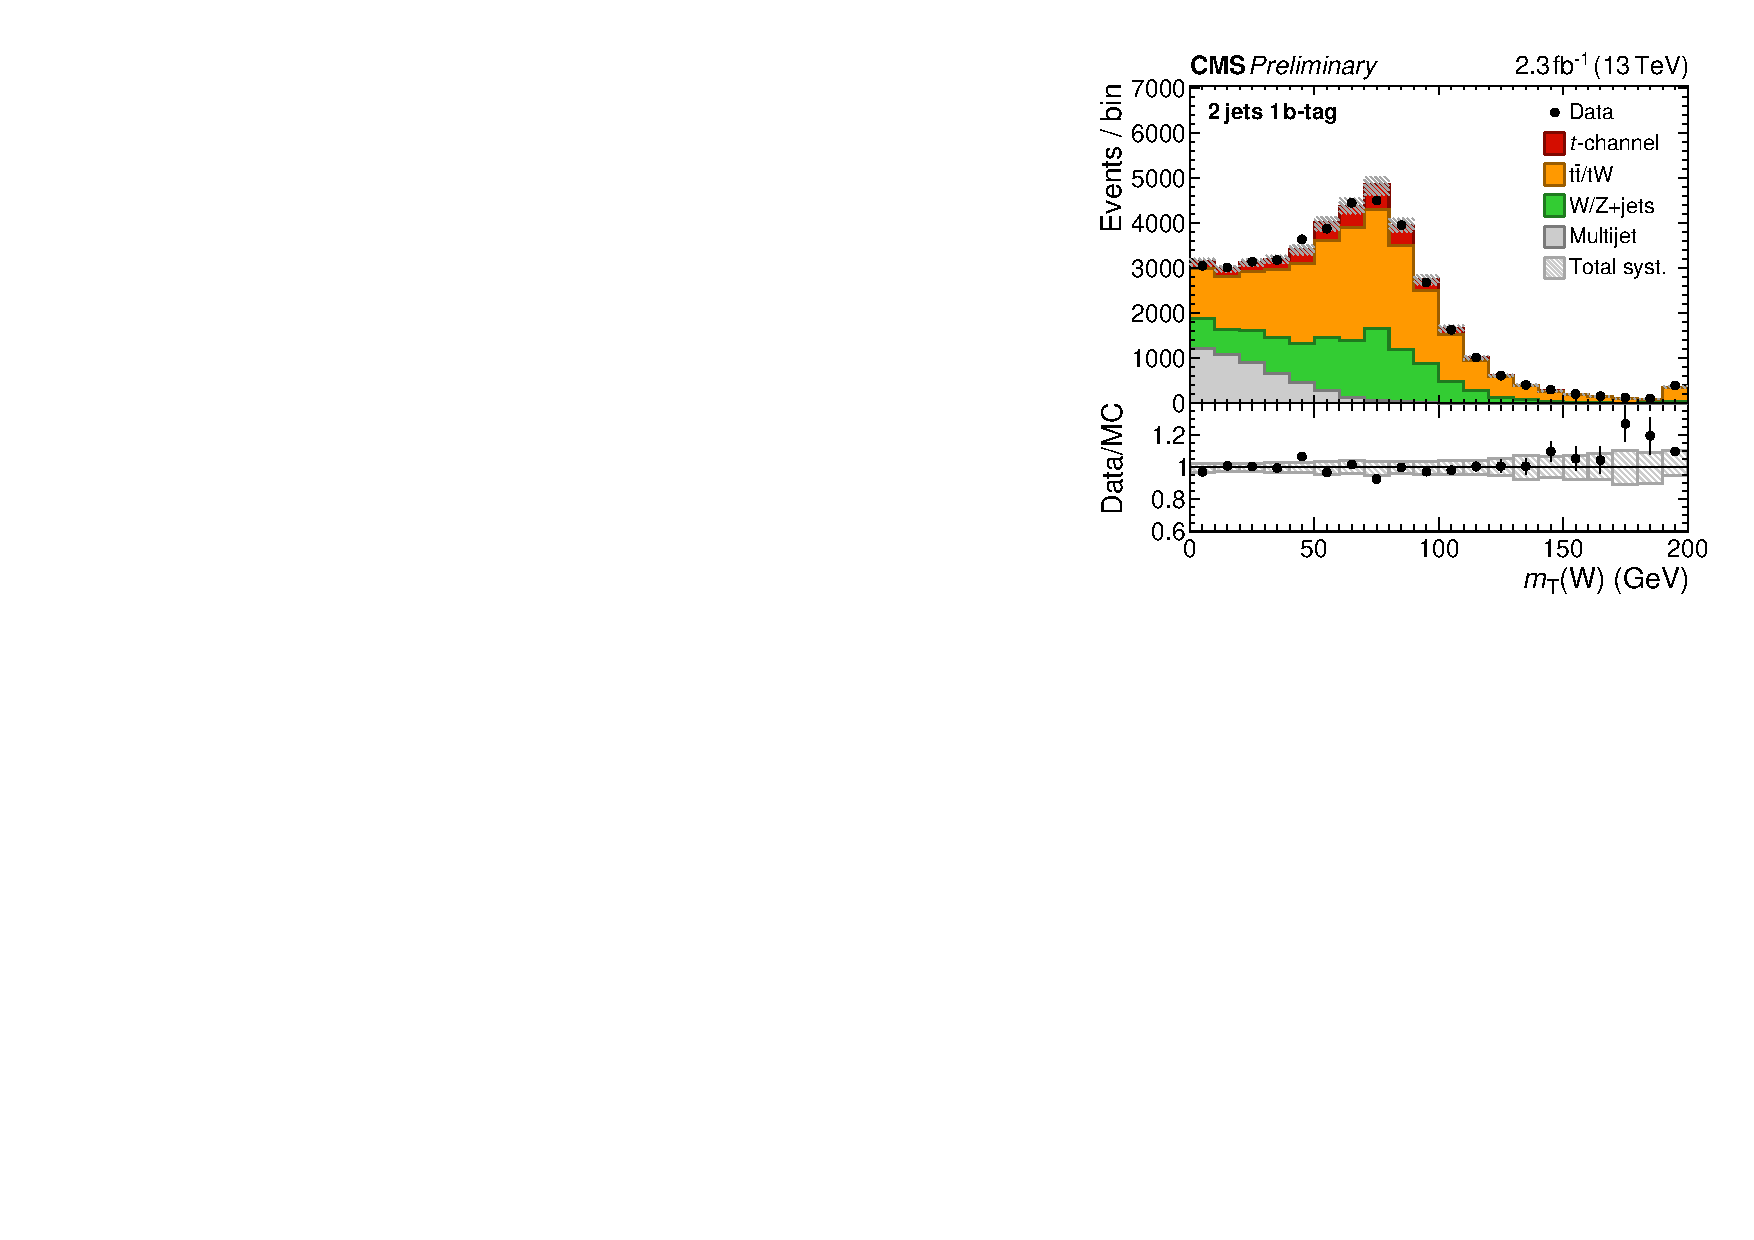
\includegraphics[width=0.48\textwidth]{figures/differential/pas/reco_mtw.pdf}}
\hspace{0.02\textwidth}
\subfloat[\label{fig:diff13-training-obs-etaj}]{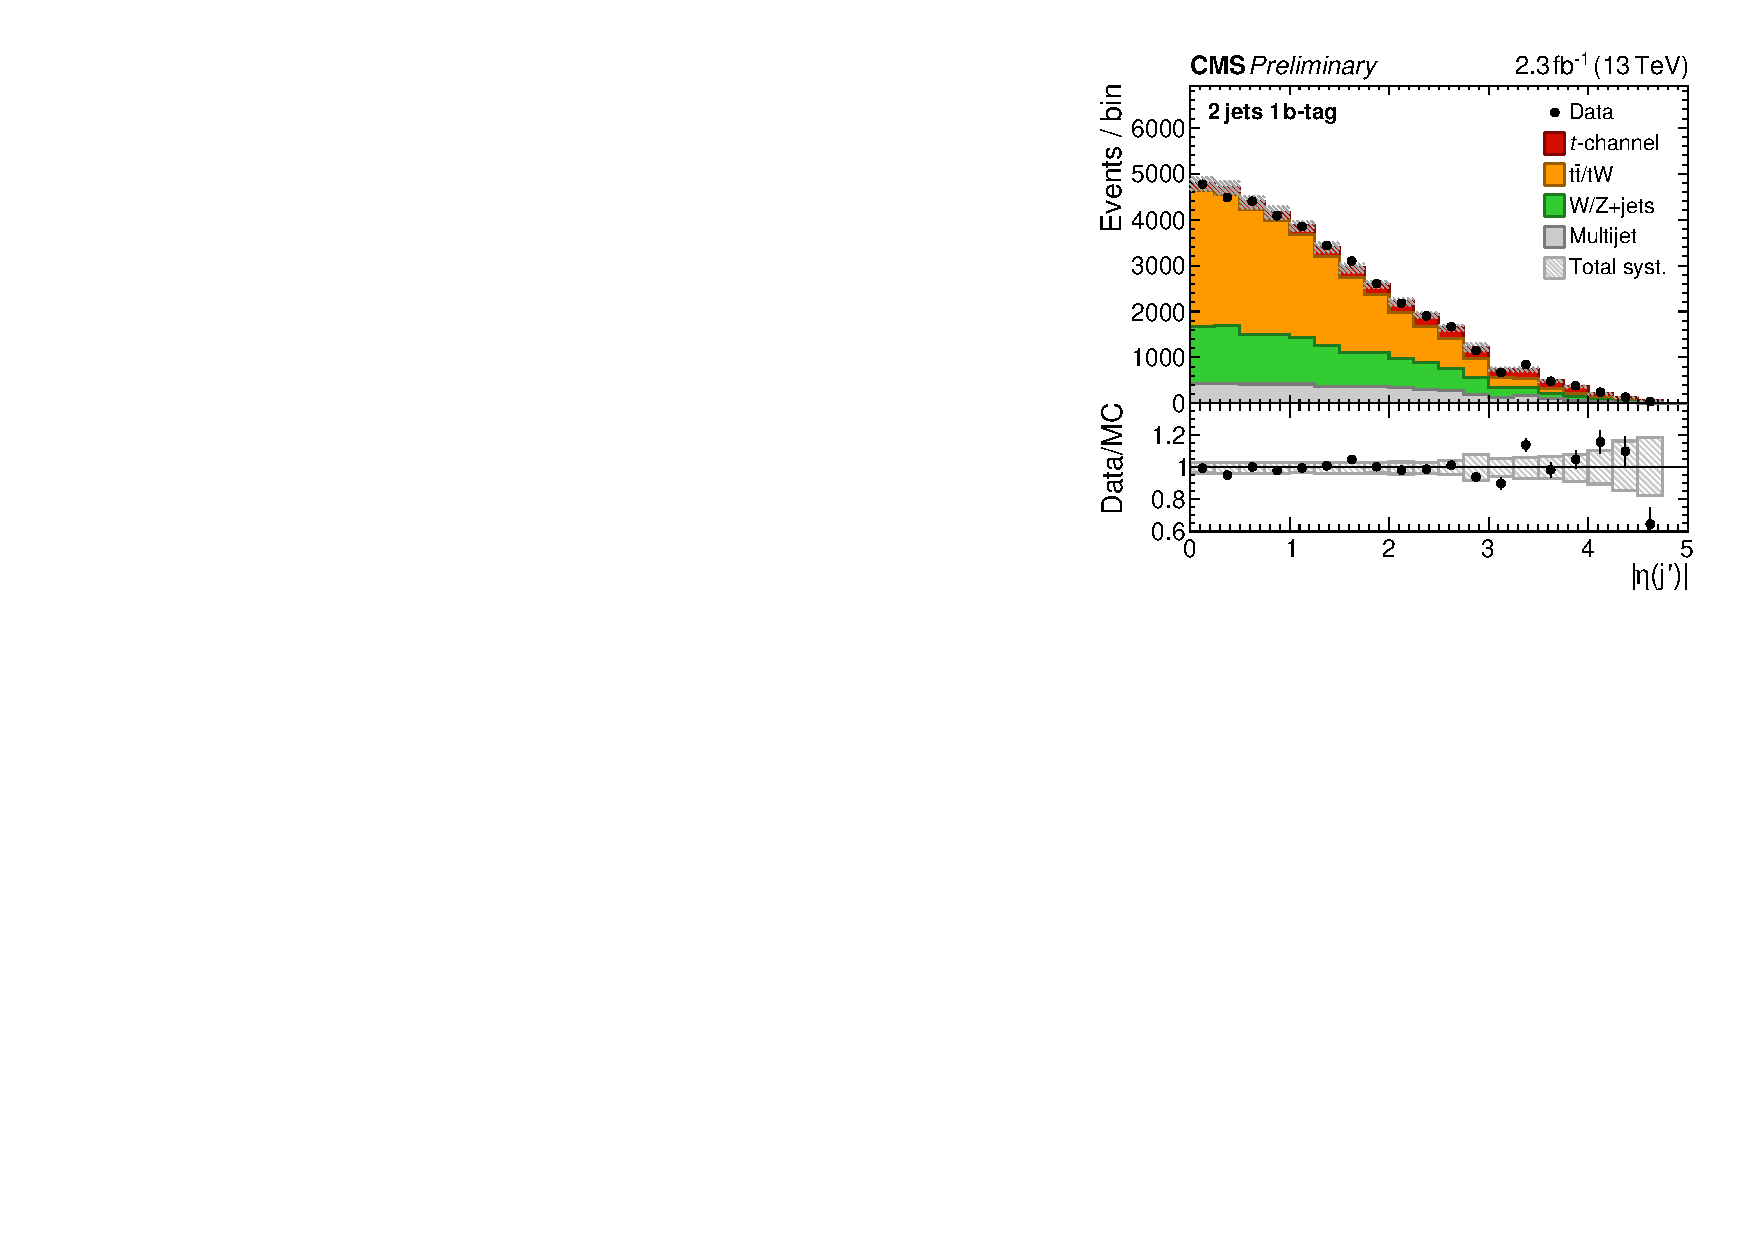
\includegraphics[width=0.48\textwidth]{figures/differential/pas/reco_etaj.pdf}}\\
\subfloat[]{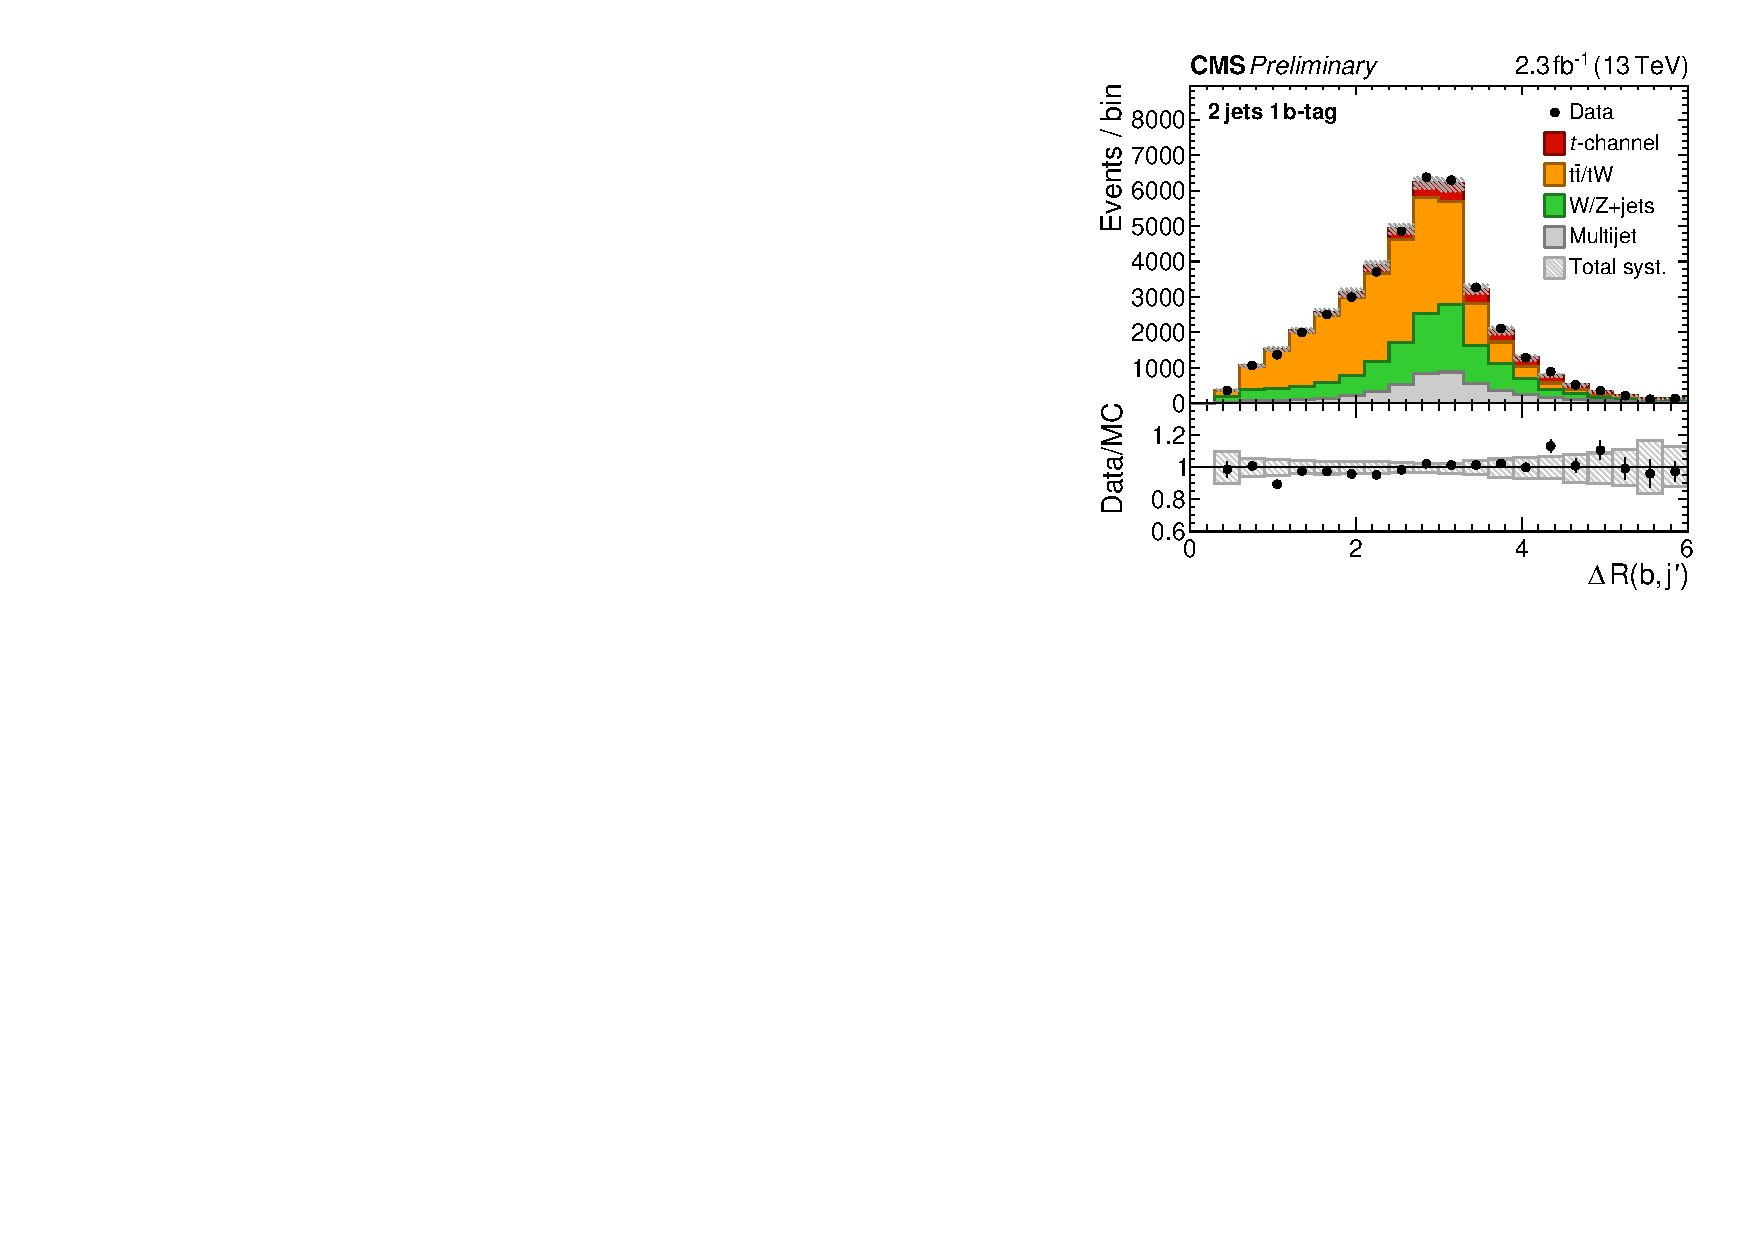
\includegraphics[width=0.48\textwidth]{figures/differential/pas/reco_dR.pdf}}
\hspace{0.02\textwidth}
\subfloat[]{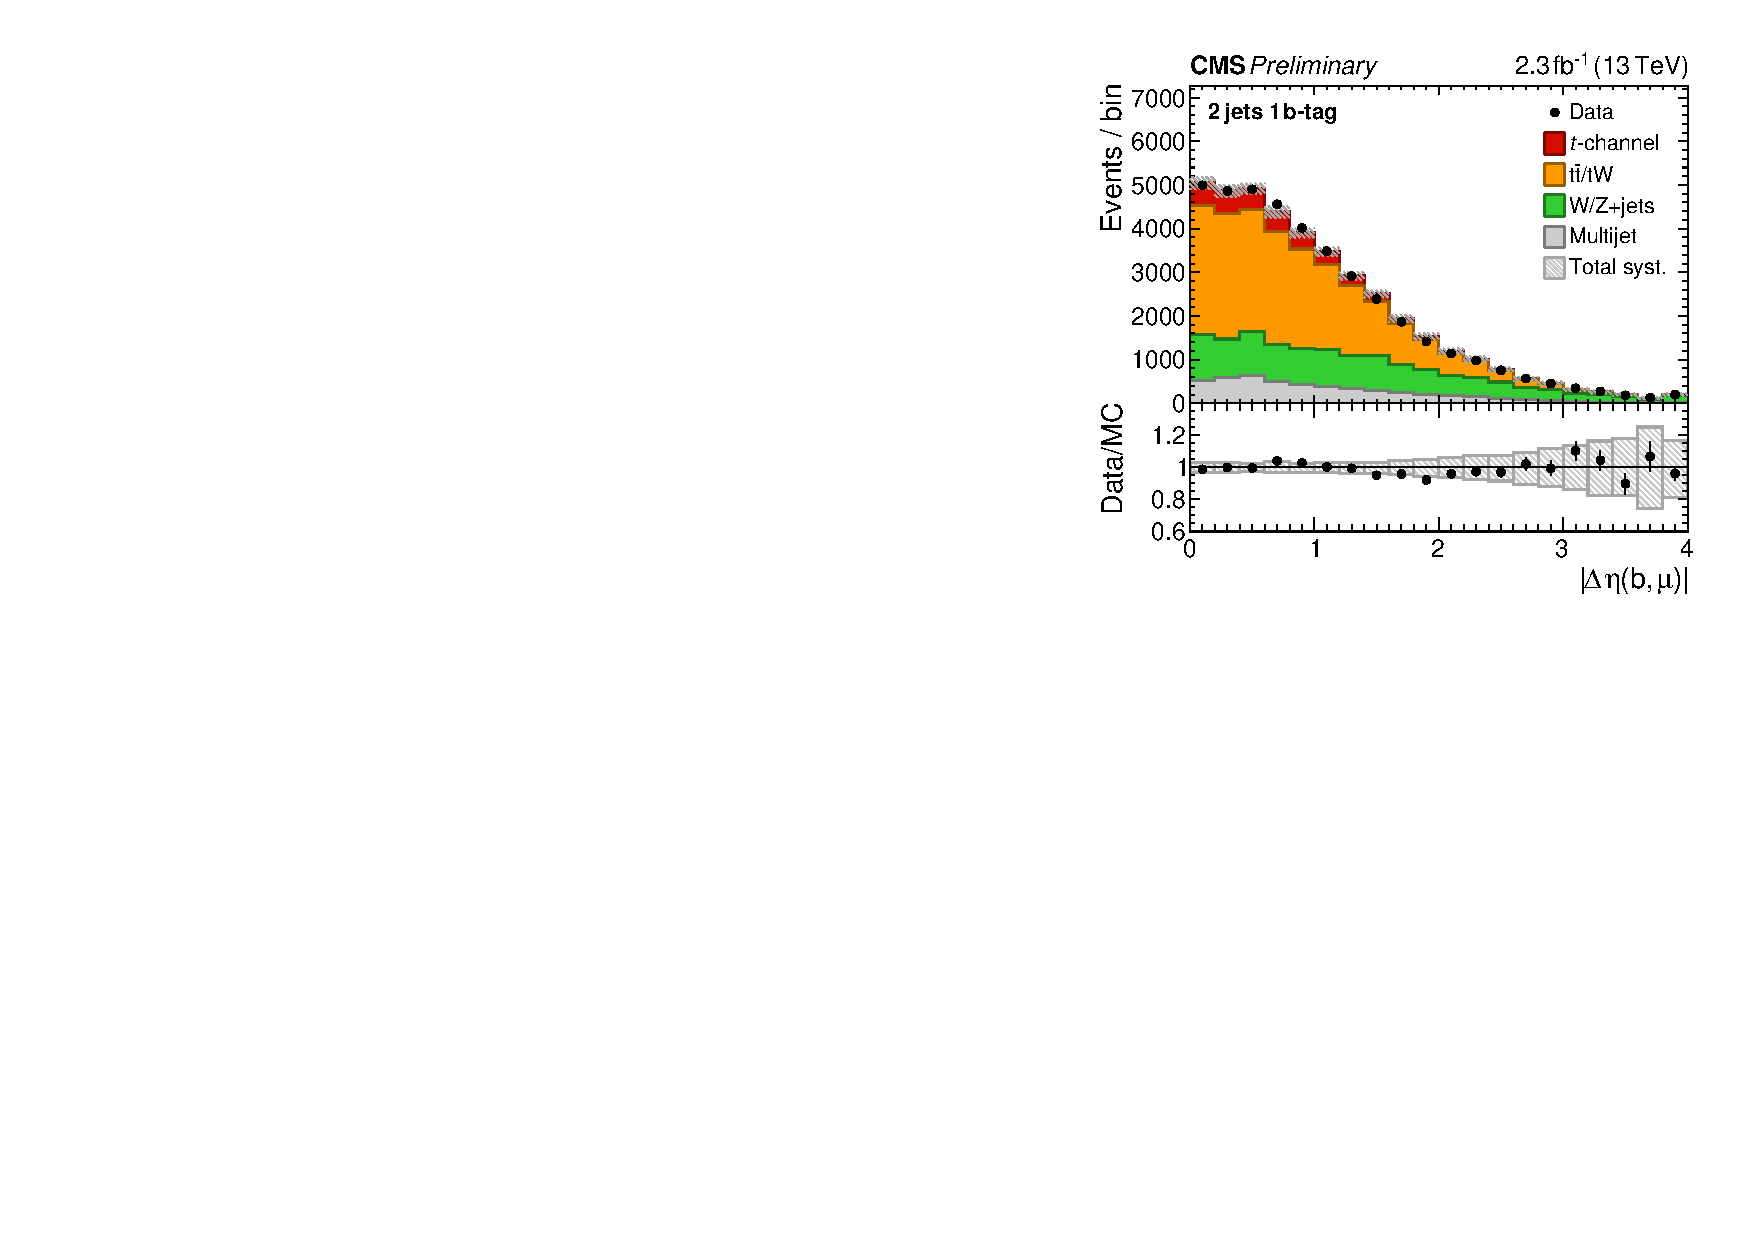
\includegraphics[width=0.48\textwidth]{figures/differential/pas/reco_dEta.pdf}}\\
\subfloat[\label{fig:diff13-bdt-raw}]{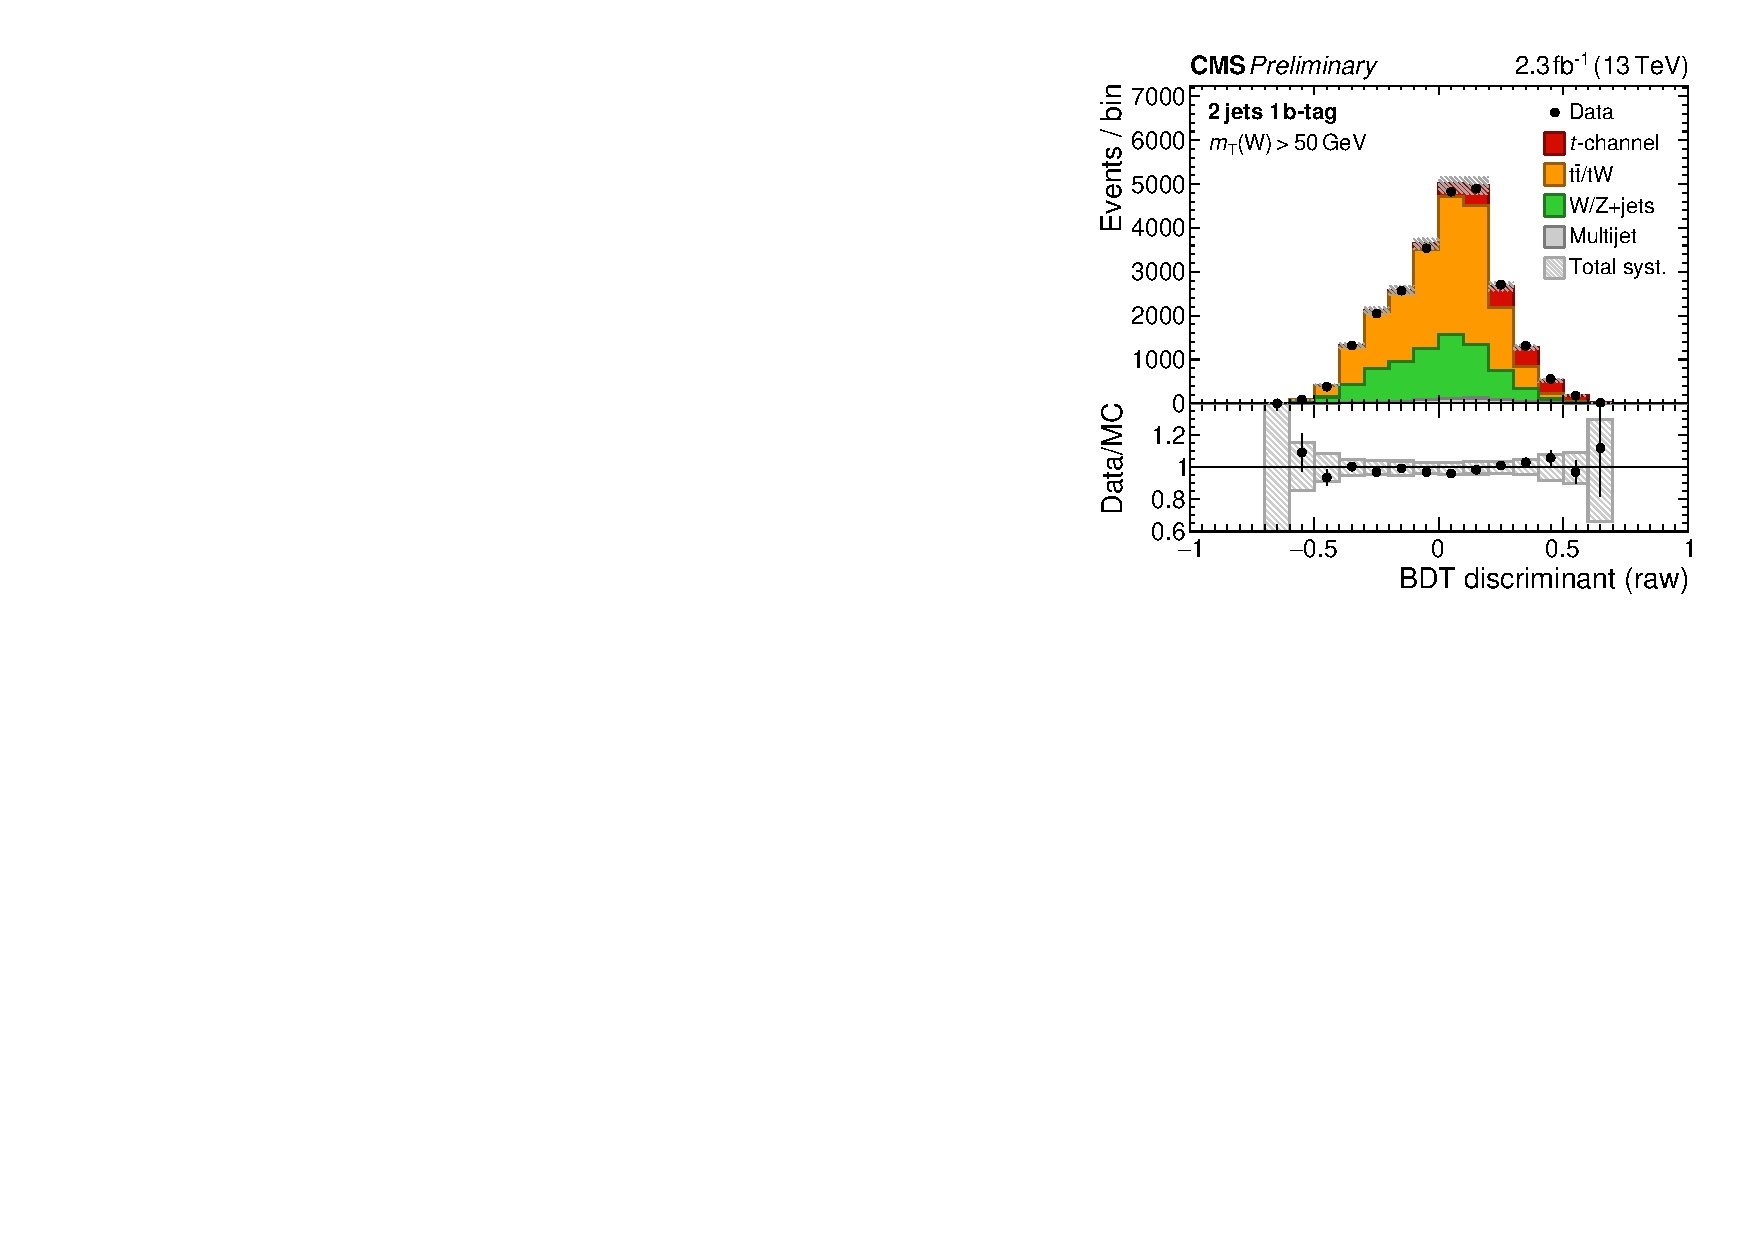
\includegraphics[width=0.48\textwidth]{figures/differential/pas/reco_BDT_unw.pdf}}
\hspace{0.02\textwidth}
\subfloat[\label{fig:diff13-bdt-mod}]{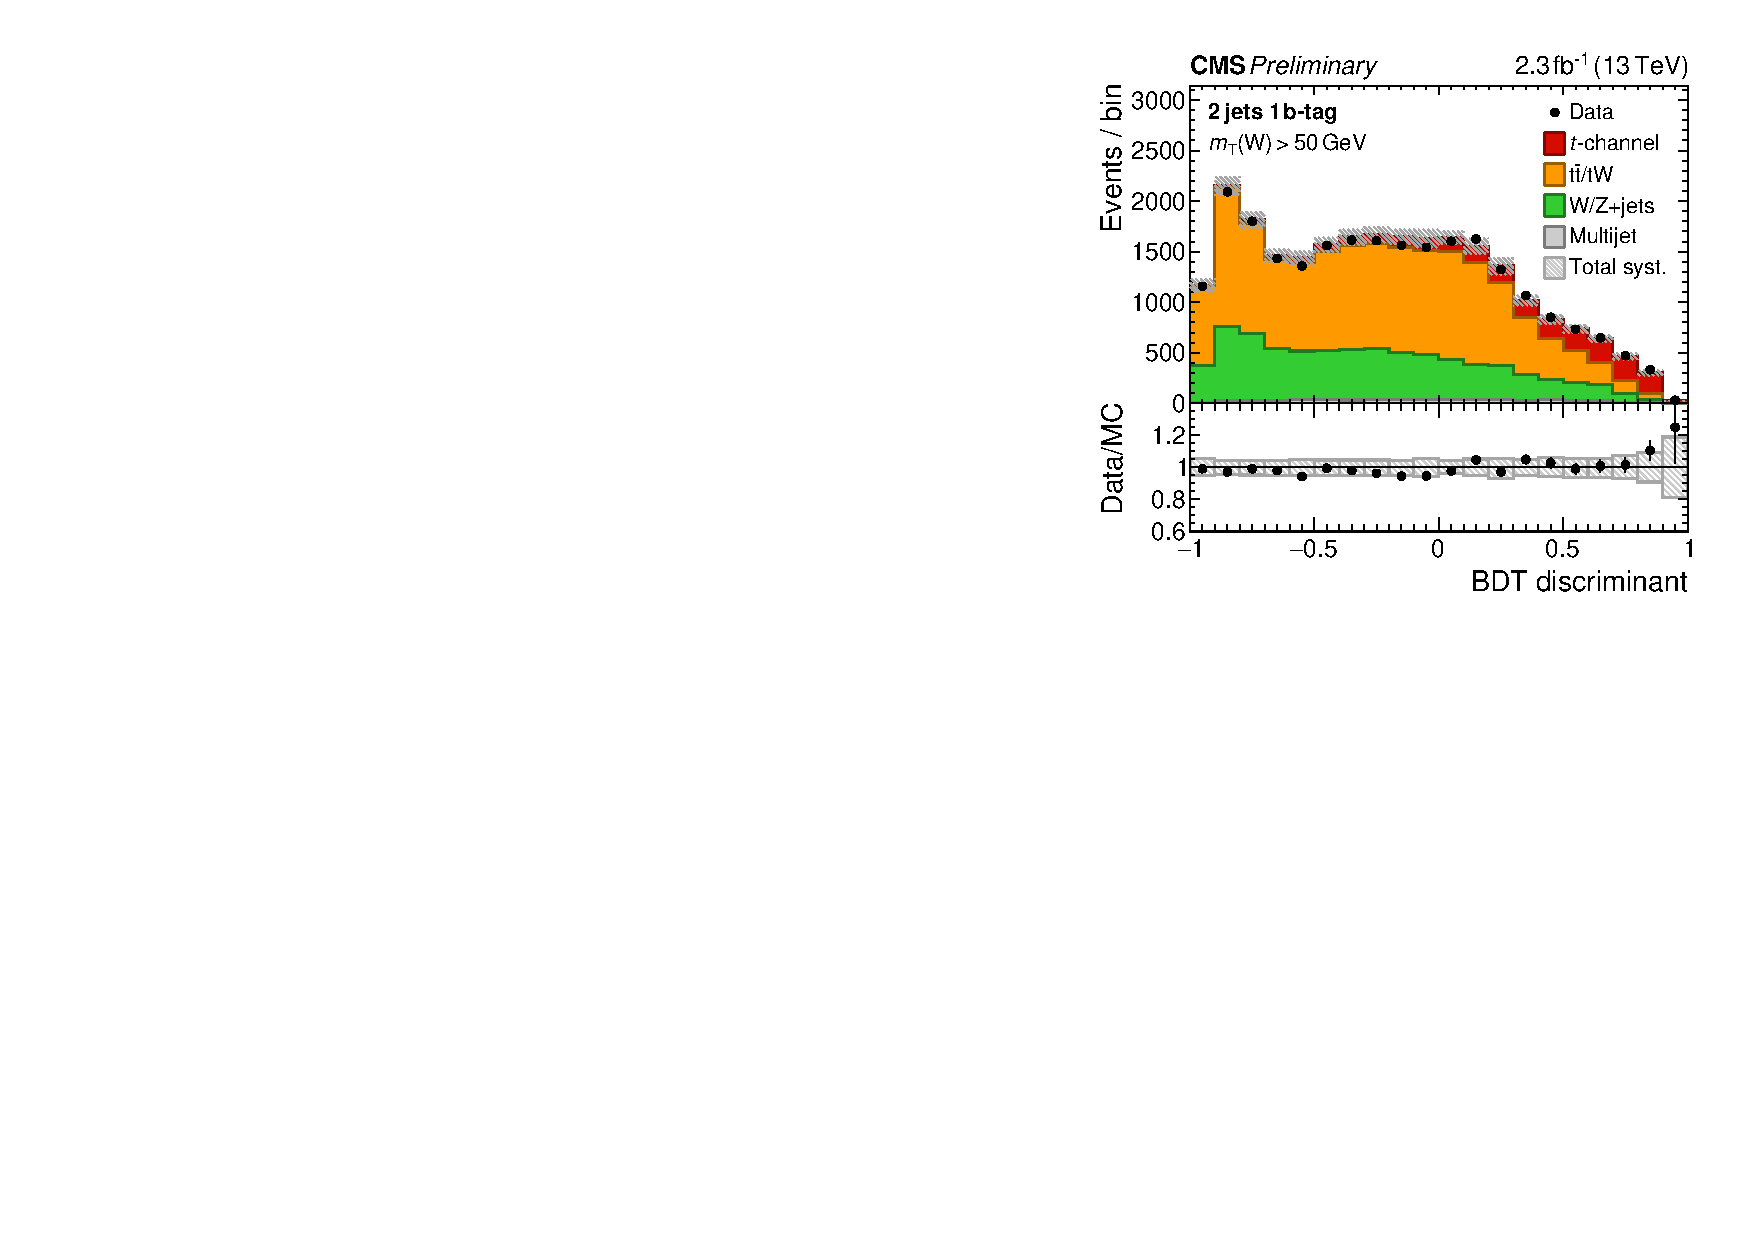
\includegraphics[width=0.48\textwidth]{figures/differential/pas/reco_BDT.pdf}}
}

The correlations between the top quark \pt, rapidity, and the \gls{bdt} input observables for $t$-channel single-top-quark events are presented in Fig.~\ref{fig:diff13-correlation-inputs}. In general, the correlations with the top quark \pt and rapidity are found to be relatively low. For the top quark rapidity the largest correlation amounts to $8\%$ with the transverse W~boson mass while for the top quark \pt a correlation of $-14\%$ is observed with the pseudorapidity of the spectator jet.

\myfigure{\label{fig:diff13-correlation-inputs}Pearson correlation coefficients between the \gls{bdt} input observables and the top quark \pt and rapidity for $t$-channel single-top-quark events.}{
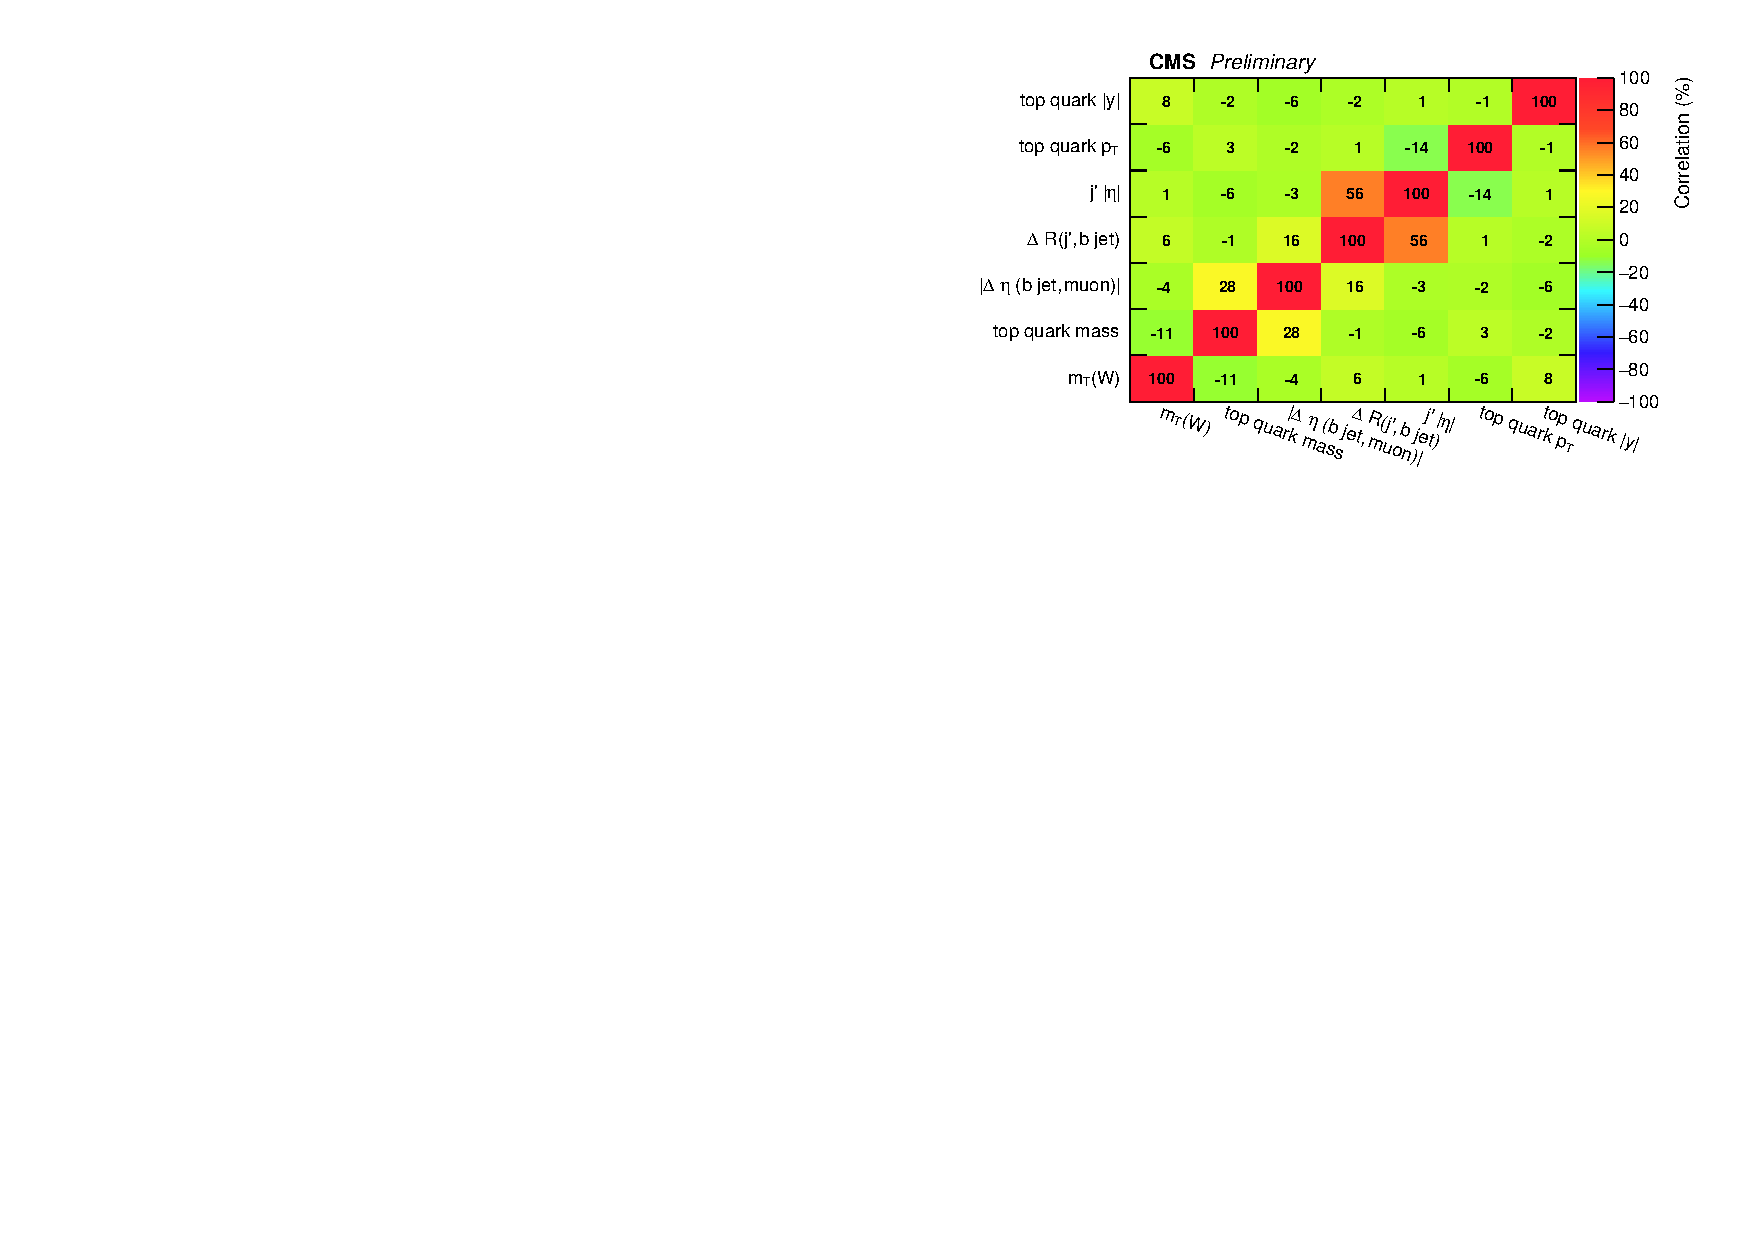
\includegraphics[width=0.8\textwidth]{figures/differential/ObsCorrelations.pdf}
}


%##############################################
\section{Signal extraction}
%##############################################
\label{sec:diff13-fit}

In past single-top-quark measurements (e.g. Refs.~\cite{Khachatryan:2015dzz,Khachatryan:2014iya,Sirunyan:2016cdg}), the contamination by multijet events is estimated following a common procedure in which an extra \gls{ml} fit to data is performed using the \mtw or \met distribution while keeping all other processes grouped together. The amount of signal events is then estimated by performing a \gls{ml} fit using a discriminating observables such as the pseudorapidity of the spectator jet or an \gls{mva} discriminant while fixing the multijet yield to the first fit result. The reason behind this two-staged fitting procedure is that the \mtw or \met shape is very sensitive to the multijet yield whereas another observable is required to provide sufficient sensitivity for breaking-down the contributions by the signal and the other backgrounds~(see also Tab.~\ref{tab:diff13-aucs}). In this measurement a novel fitting strategy, outlined in the following, has been developed which allows to simultaneously estimated the amount of signal, the contamination by multijet events, and the contributions by the other backgrounds processes by performing only a single \gls{ml} fit. The log-likelihood of the fit can be written as

\begin{equation}
\ln\big(\mathsf{L}_\mathrm{total}\big)=\ln\big(\mathsf{L}^\mathrm{2j1t}_\mathrm{Poi.}\big)+\ln\big(\mathsf{L}_\mathrm{Poi.}^\mathrm{3j1t}\big)+\ln\big(\mathsf{L}_\mathrm{Poi.}^\mathrm{3j2t}\big)+\mathrm{constraints}\,.
\end{equation}

in which the Poisson terms per region $X=(\mathrm{2j1t, 3j1t, 3j2t})$ are given by

\begin{equation}
\ln\Big(\mathsf{L}^{X}_\mathrm{Poi.}\big(\vec{d}^{\,X}|\,\vec{p}^{\,X}\big)\Big)=\sum_{i}^\mathrm{bins}\Big(d_{i}^{X}\ln p_{i}^{X}-p_{i}^{X}\Big)+\mathrm{const.}\,,
\end{equation}

where $d_{i}$ denotes the amount of data events and $p_{i}$ the prediction per bin $i$. The predictions per region can be expressed as

\begin{subequations}
\begin{align}
\vec{p}^{\,X}~=\hphantom{+}&~\beta_{t\mathrm{\mbox{-}channel}}\cdot \vec{T}_{t\mathrm{\mbox{-}channel}}^{\,X}\\
+&~\beta_\mathrm{top~bkg.}\cdot\Big(\vec{T}^{\,X}_{\ttbar}+\vec{T}^{\,X}_\mathrm{tW}\Big)\\
+&~\beta_\mathrm{W/Z\mbox{+}jets}\cdot\Big(\vec{T}^{\,X}_{\wjets}+\vec{T}^{\,X}_{\zjets}\Big)\\
+&~\beta_\mathrm{multijet}^{X}\cdot \vec{T}^{\,X}_\mathrm{multijet}\,,
\end{align}
\end{subequations}

where $\vec{T}_{j}$ denotes a template of a process whose normalization is modified by a corresponding scale factor $\beta_{j}$. In this fit, background processes containing genuine top quarks~(\ttbar, tW) have been grouped together as well as the electroweak processes~(\wjets, \zjets). A log-normal prior with an uncertainty of $\pm10\%$ is used to constrain the normalization of the top quark background. For the W/Z+jet background a conservative larger prior with a width of $\pm30\%$ is assumed. The normalization of the multijet templates are kept almost unconstrained using independent scale factors per region with an uncertainty of $\pm100\%$ on their yield. No constraint on the signal scale factor is applied.

A compound distribution is utilized for fitting using the transverse W~boson mass distribution for events with $\mtw<50~\GeV$ and the distribution of the trained \gls{bdt} discriminant otherwise. A comparison of the different template shapes for both distributions in 2j1t as fitted is presented in Fig.~\ref{fig:diff13-fittemplates}. Only five bins are used for the \mtw distribution and 15 for the \gls{bdt} distribution to reduce the impact by the limited simulation statistics on the result. Since the \ttbar and \wjets shapes appear to be very similar, the two \ttbar control regions~(3j1t, 3j2t) are fitted simultaneously as well providing an additional handle on the \ttbar yield. 

\myfigure{\label{fig:diff13-fittemplates}Shapes of the \gls{ml} fit templates in 2j1t region.}{
\subfloat[]{\adjincludegraphics[height=4.8cm,trim={0 0 {0.16\width} 0},clip]{figures/differential/fitshape/comp_2j1t_2j1t_mtw_qcdmtwinv_nol.pdf}}
\subfloat[]{\adjincludegraphics[height=4.8cm,trim={0 0 {0.\width} 0},clip]{figures/differential/fitshape/comp_2j1t_2j1t_BDT_adaboost04_minnode001_maxvar3_ntree1000_invboost_binned_qcdmtw.pdf}}
}

The estimated yields per process in the 2j1t region after the event selection are listed in Tab.~\ref{tab:diff13-fit-result}. Extrapolated yields are also given in a multijet-depleted region and in a signal-enriched region for reference, where in the latter a \gls{sb} of about one is obtained. The correlations between the estimated scale factors are presented in Fig.~\ref{fig:diff13-fit-correlation}. Overall the absolute value of the correlation does not exceed 34\% with the exception of the 3j2t multijet scale factor for which the corresponding template contributes however only 2\% of events in the 3j2t region in total compared to the other processes. In particular the anticorrelation between the \wjets and \ttbar yields amounts to only -33\% through the new fitting strategy which marks a significant reduction compared to the fit result in the top quark polarization measurement where an anticorrelation of $-75\%$ was achieved~(Sec.~\ref{sec:polarization-fit}).

\mytable{\label{tab:diff13-fit-result}Estimated event yields in the 2j1t region: after the event selection; for events with $\mtw>50~\GeV$; in a signal-enriched phase space defined by $\mtw>50~\GeV$ and $\bdt>0.6$\,.}{
\begin{tabular}{@{}l l r@{$\pm$}l c r@{$\pm$}l c r@{$\pm$}l@{}}
\toprule
Process &\hspace*{0.3cm}&\multicolumn{8}{c@{}}{Event yields}  \\
\cmidrule{3-10}
&&\multicolumn{2}{c}{Selection} &\hspace*{0.2cm}& \multicolumn{2}{c}{$\mtw>50~\GeV$} &\hspace*{0.2cm}& \multicolumn{2}{c@{}}{Signal-enriched}\\
\midrule
tW              &&\hspace*{0.1cm} 2001&14      &&\hspace*{0.5cm} 1343&12       &&\hspace*{0.6cm} 32&2\\
\ttbar          && 19037&22     && 12960&18      && 353&3\\
W+heavy flavor  && 6825&57      && 4807&49       && 189&11 \\
W+light flavor  && 2395&40      && 1684&34       && 71&7 \\
\zjets          && 1534&24      && 664&16        && 23&3 \\
Multijet        && 4881&18      && 561&3         && 38&1\\
Signal          && 3385&5       && 2351&4        && 700&2\\
\midrule
Total expected  && 40057&80     && 24369&66      && 1407&13\\
Data            && 40432&201    && 24417&156     && 1482&38 \\
\bottomrule
\end{tabular}
}

\myfigure{\label{fig:diff13-fit-correlation}Correlations between the estimated scale factors.}{
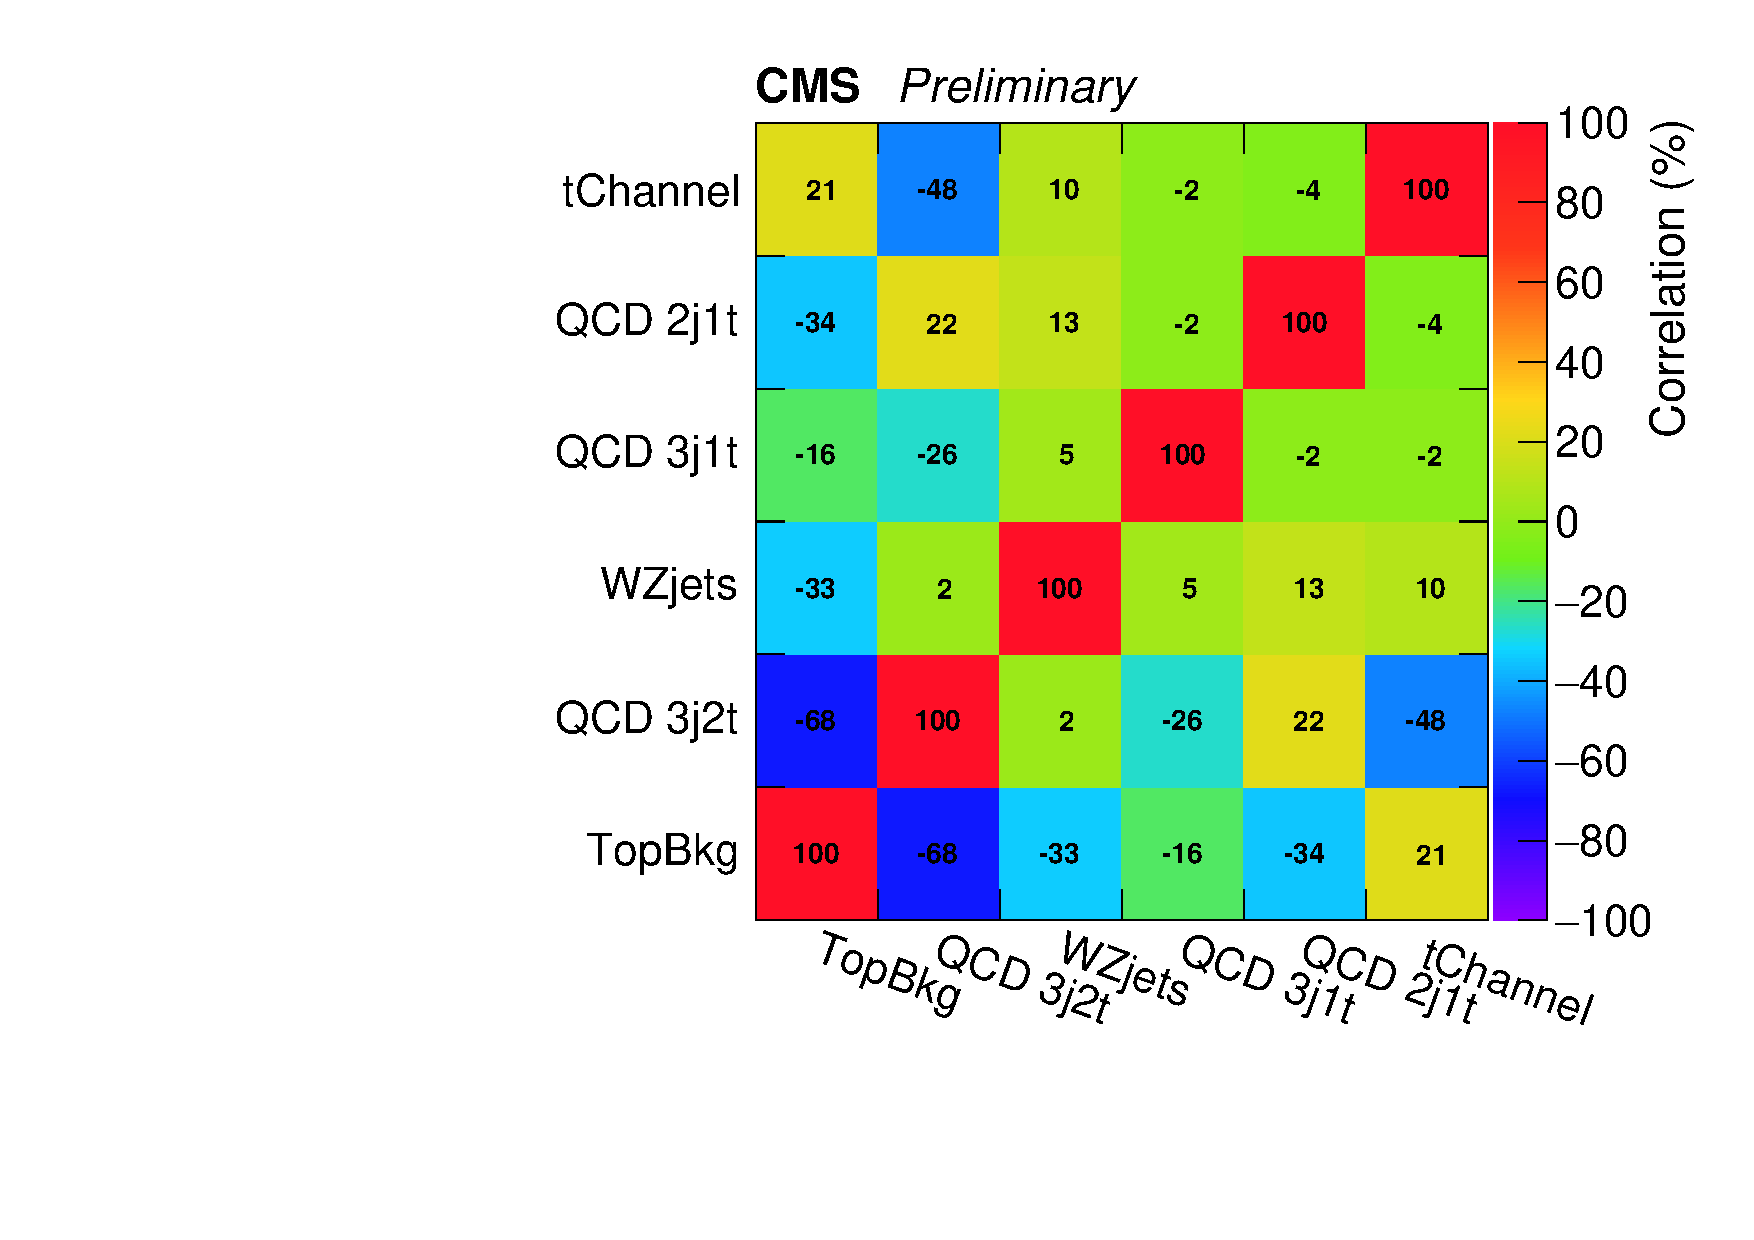
\includegraphics[width=0.6\textwidth]{figures/differential/fitCorrelations.pdf}
}


Besides the inclusive \gls{ml} fit, multiple fits are performed in addition utilizing the same strategy while being however restricted to events within a certain interval of the reconstructed top quark \pt or rapidity. Estimating separate scale factors in these intervals yields several advantages for the measurement as listed in the following.

\begin{itemize}
\item The estimated scale factors allow to calculate the yield of the signal as a function of the top quark \pt and rapidity directly. Thus, contributions from background processes do not have to be explicitly subtracted from data prior to the unfolding. This new approach mitigates also the impact of the limited simulation statistics on the result since the corresponding uncertainty is profiled in the fit by the \acrlong{bb} method as detailed in Sec.~\ref{sec:technique-fitting}.

\item In the top quark polarization measurement a lengthy procedure was required to obtain an optimal signal-enriched region during which the working point of a 
trained \bdt was scanned while evaluating the impact of the systematic uncertainties on the result using pseudo-data (Sec.~\ref{sec:polarization-optimization}). In this measurement, the estimated scale factors reflect directly the amount of signal and background events after the event selection. Thus, performing an optimization for finding a signal-enriched region is not required.

\item Residual differences in the background shapes may still be present in the signal region although their modeling has been validated extensively in control regions. Furthermore, the \gls{bdt} itself may introduce a bias towards the \gls{sm} prediction because only a sample of \gls{sm} $t$-channel single-top-quark events is used for its training. In the multi-fit approach potential differences and biases can be however profiled per bin of the measurement which thus mitigates their impact.
\end{itemize}


The results of the separate \gls{ml} fits in bins of the top quark \pt and rapidity are presented in Fig.~\ref{fig:diff13-individual-fits}. The depicted binning scheme for both observables is introduced in Sec.~\ref{sec:diff13-unfolding} below. Overall, the estimated scale factors per process agree with each other within the shown statistical uncertainties of the fit. The only exception is the first top quark \pt bin where an undershoot of signal is observed with respect to the \gls{sm} expectation.

\myfigure{\label{fig:diff13-individual-fits}Scale factors of the process yields with respect to the \gls{sm} expectations as a function of the top quark (a)~transverse momentum and (b)~rapidity. The vertical bars denote the statistical uncertainties on the yields. For multijet events only the scale factors with respect to the normalization from the sideband region in the 2j1t region are shown. The dashed vertical lines mark the bin edges.}{
\subfloat[]{\adjincludegraphics[height=4.8cm,trim={0 0 {0.16\width} 0},clip]{figures/differential/fitshape/multi_top_pt_nol.pdf}}
\subfloat[]{\adjincludegraphics[height=4.8cm,trim={0 0 {0.\width} 0},clip]{figures/differential/fitshape/multi_top_y.pdf}}
}


%##############################################
\section{Validation}
%##############################################

Before the unfolding is carried out, the distributions of the top quark \pt and rapidity are validated. Figure~\ref{fig:diff13-top-reco} shows the corresponding distributions in a signal-depleted and in a signal-enriched phase space. These are defined by selecting events with either $\bdt<0$ or $\bdt>0.6$ respectively while in addition requiring only events with $\mtw>50~\GeV$ to suppress contributions from multijet production. A good agreement is observed in the signal-depleted phase space for both observables within uncertainties. For the top quark rapidity distribution a good description of data by the templates is also observed in the signal-enriched region. The top quark \pt distribution in data displays however a somewhat harder spectrum compared to the expectation. In particular the prediction in the first \pt bin overestimates the observed amount of events in data which also confirms the result obtained from the separate \gls{ml} fits presented in Fig.~\ref{fig:diff13-individual-fits}.

\myfigure{\label{fig:diff13-top-reco} Distributions of the (top row)~top quark \pt and (bottom row)~rapidity in (left column)~a signal-depleted and (right-column)~a signal-enriched phase space defined by $\bdt<0$ and $\bdt>0.6$ respectively after requiring only events with $\mtw>50~\GeV$ to suppress contributions from multijet production. The hatched bands reflect the total systematic uncertainties. The figures are taken from Ref.~\cite{CMS-PAS-TOP-16-004}.}{
\subfloat[]{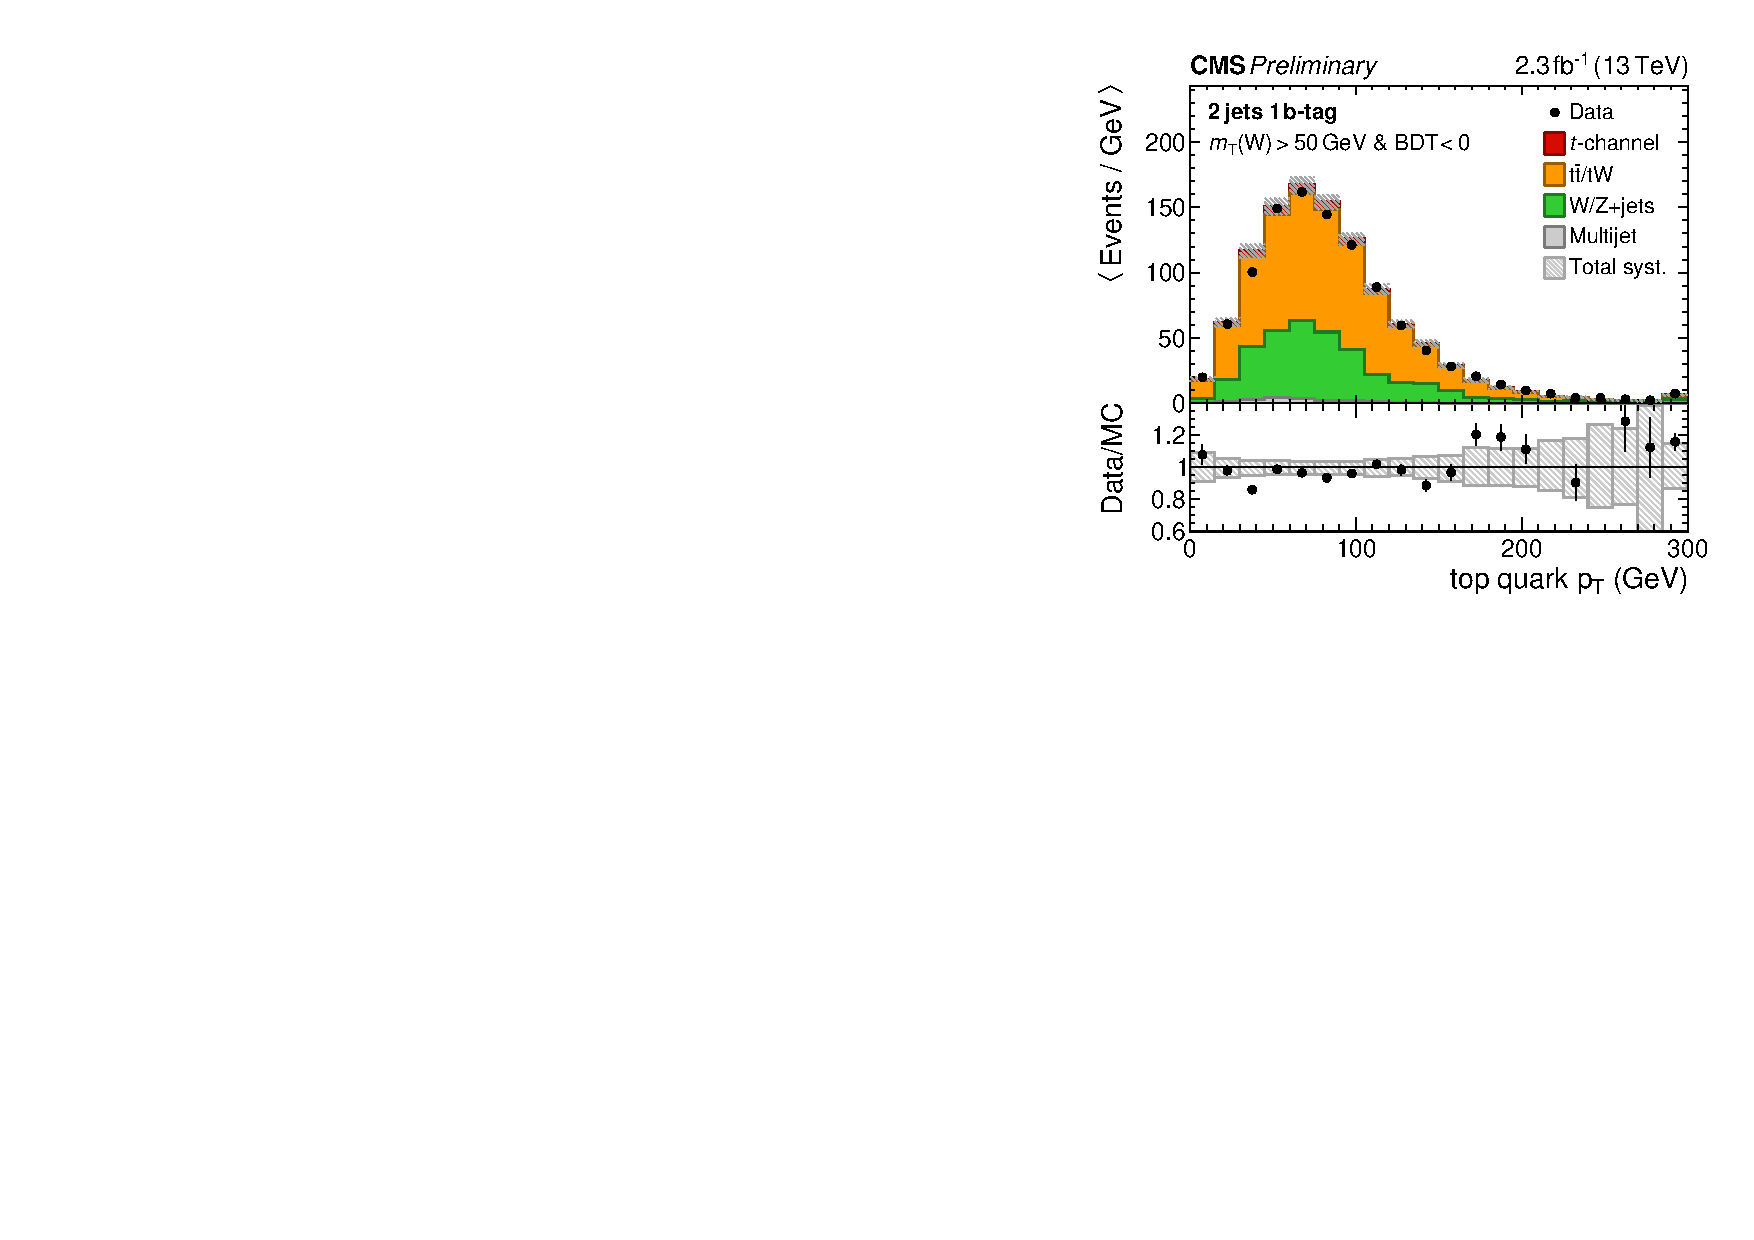
\includegraphics[width=0.48\textwidth]{figures/differential/pas/reco_toppt_bdtinv.pdf}}
\hspace{0.02\textwidth}
\subfloat[]{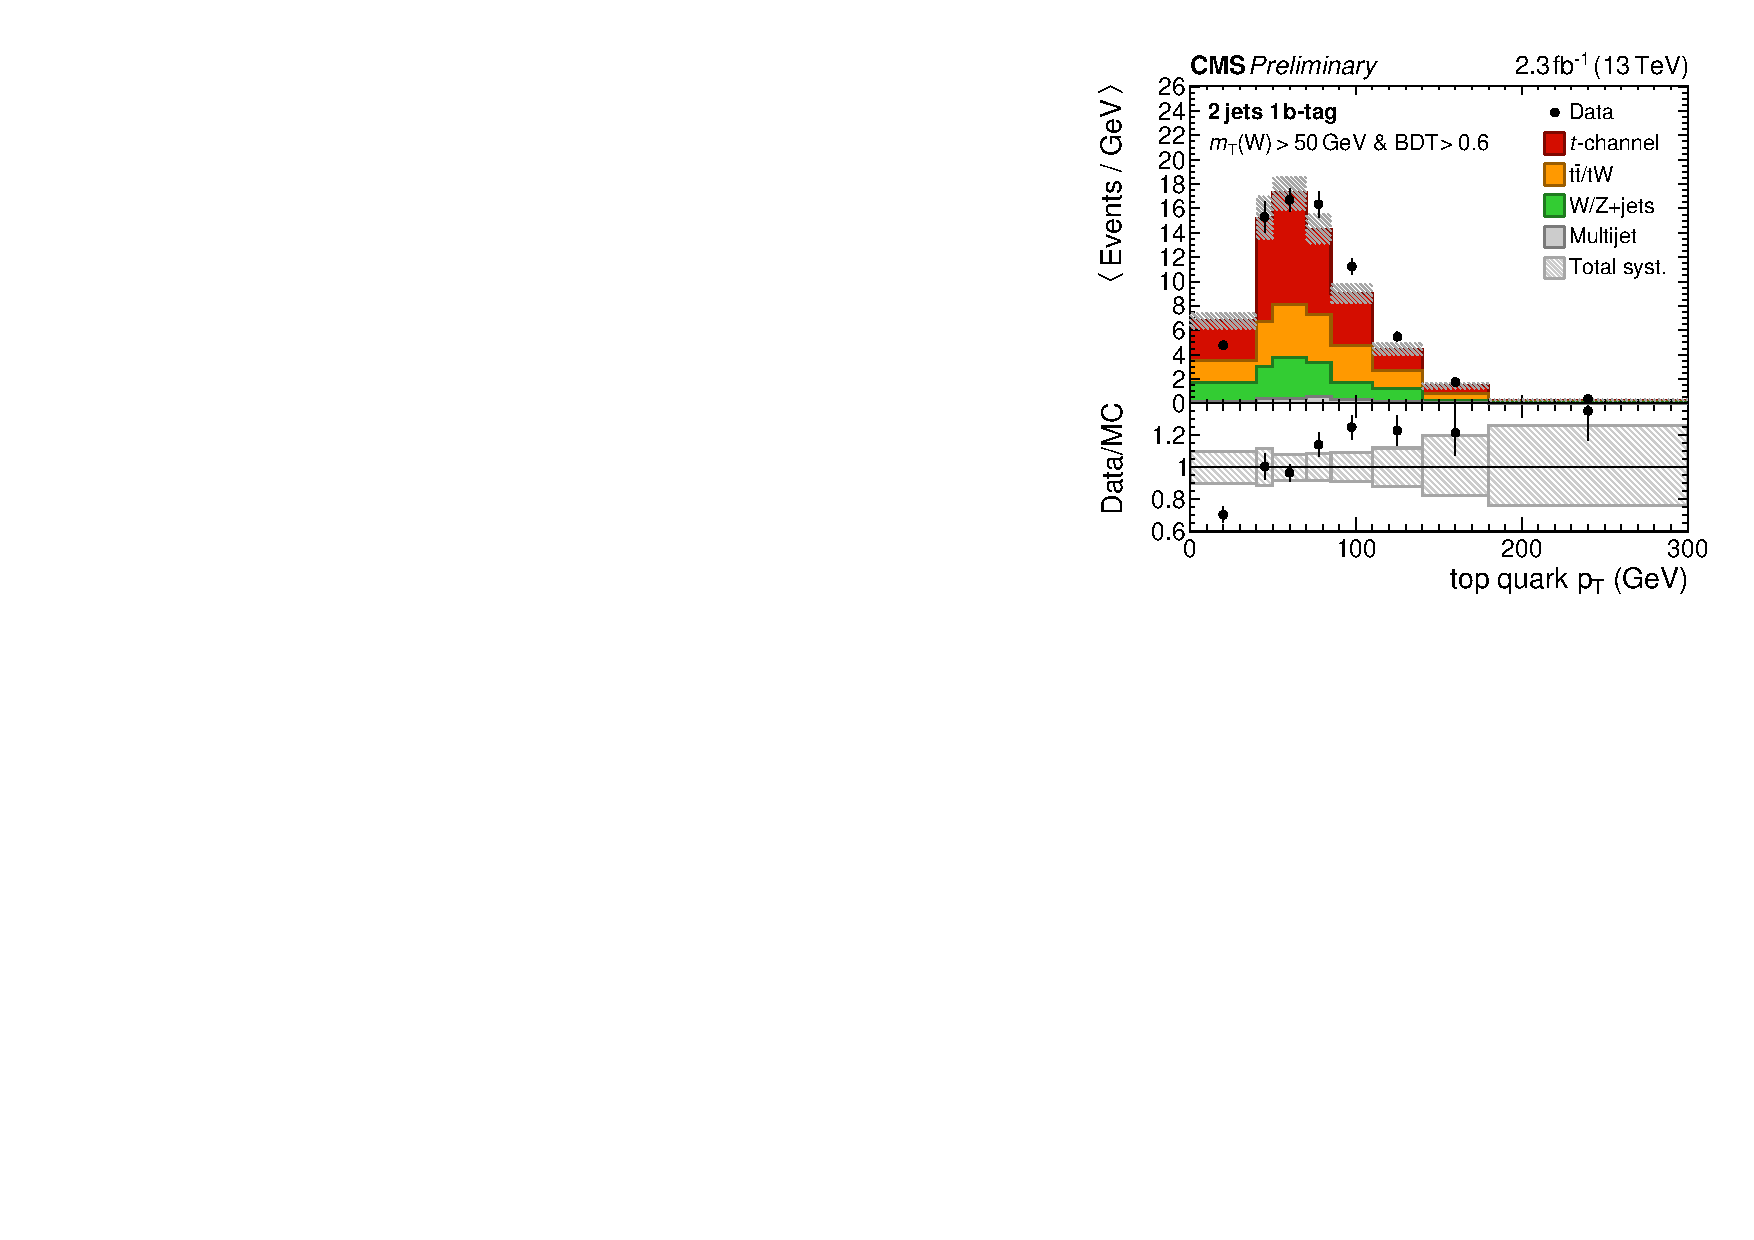
\includegraphics[width=0.48\textwidth]{figures/differential/pas/reco_toppt_bdt.pdf}}\\
\subfloat[]{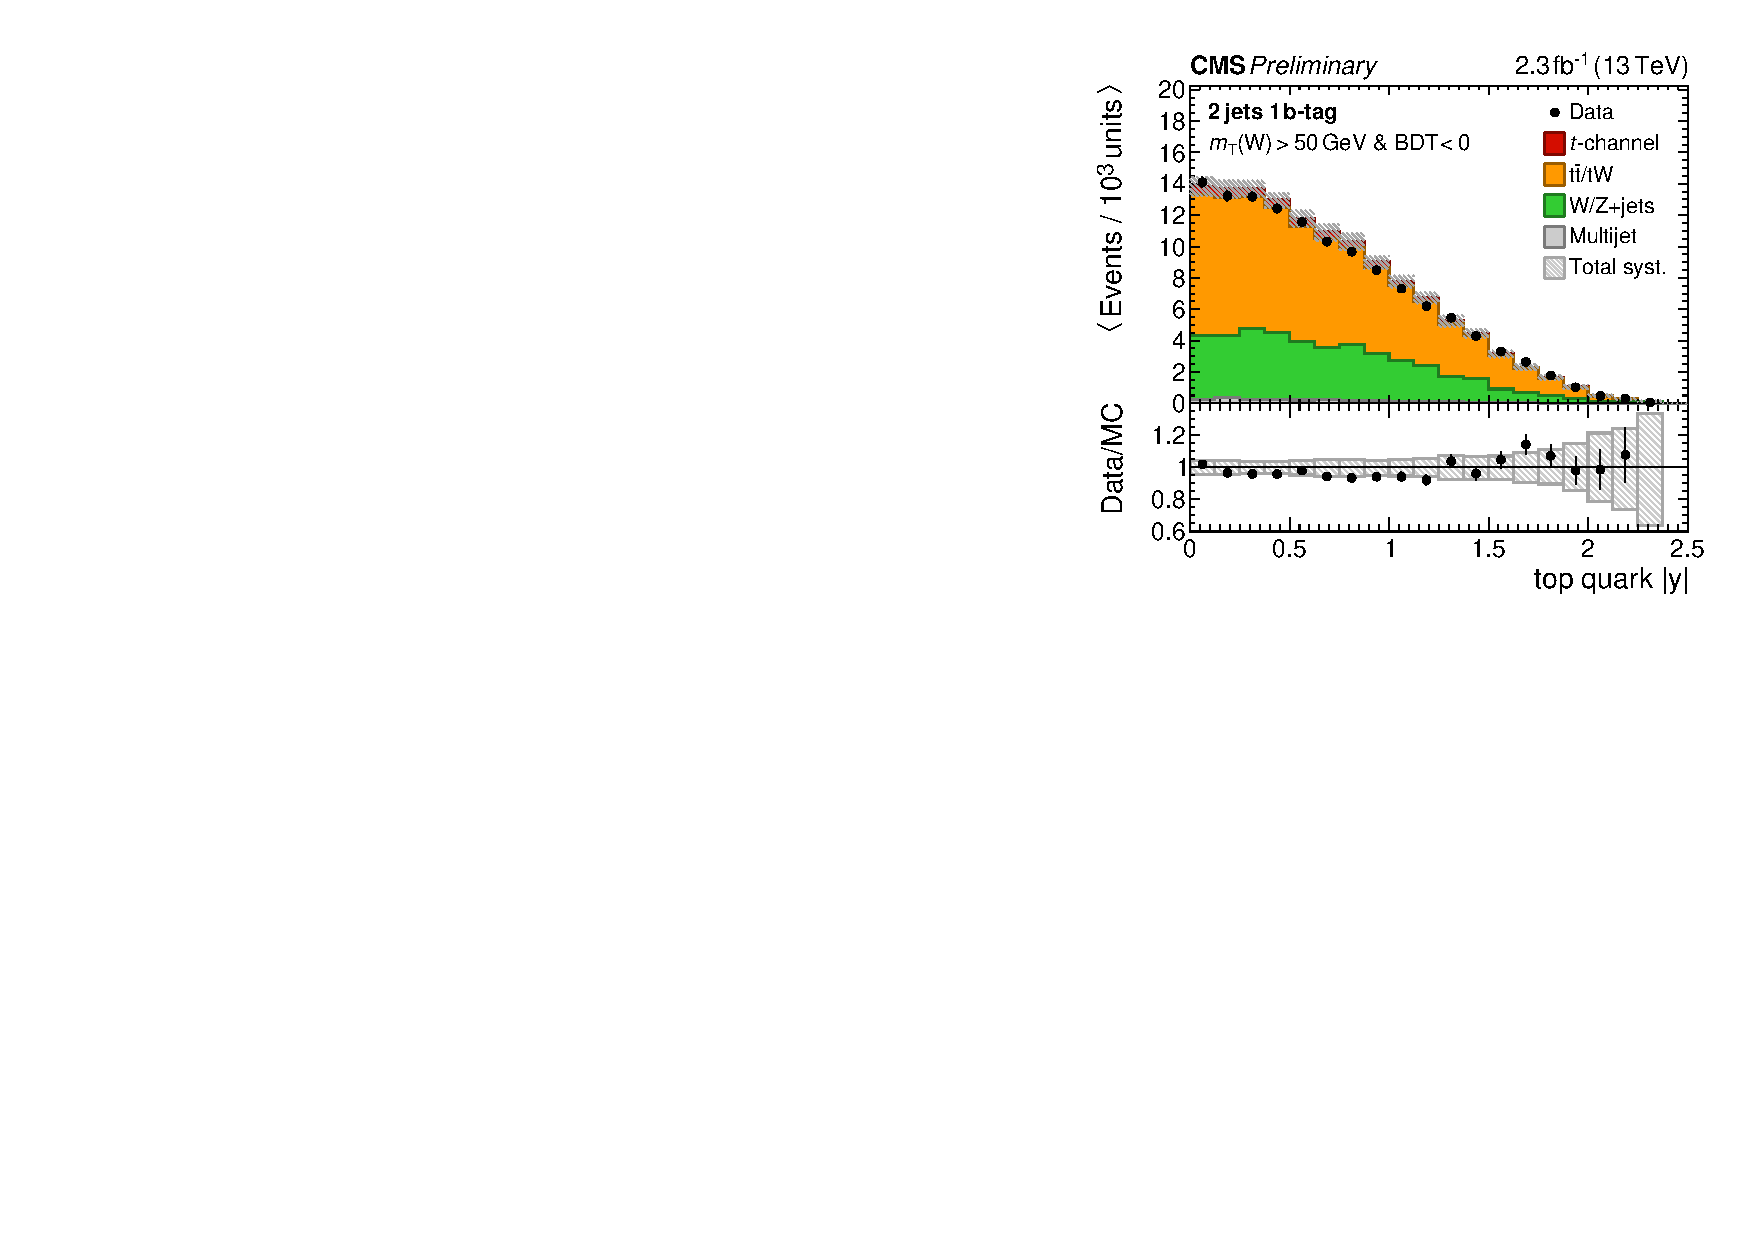
\includegraphics[width=0.48\textwidth]{figures/differential/pas/reco_topy_bdtinv.pdf}}
\hspace{0.02\textwidth}
\subfloat[]{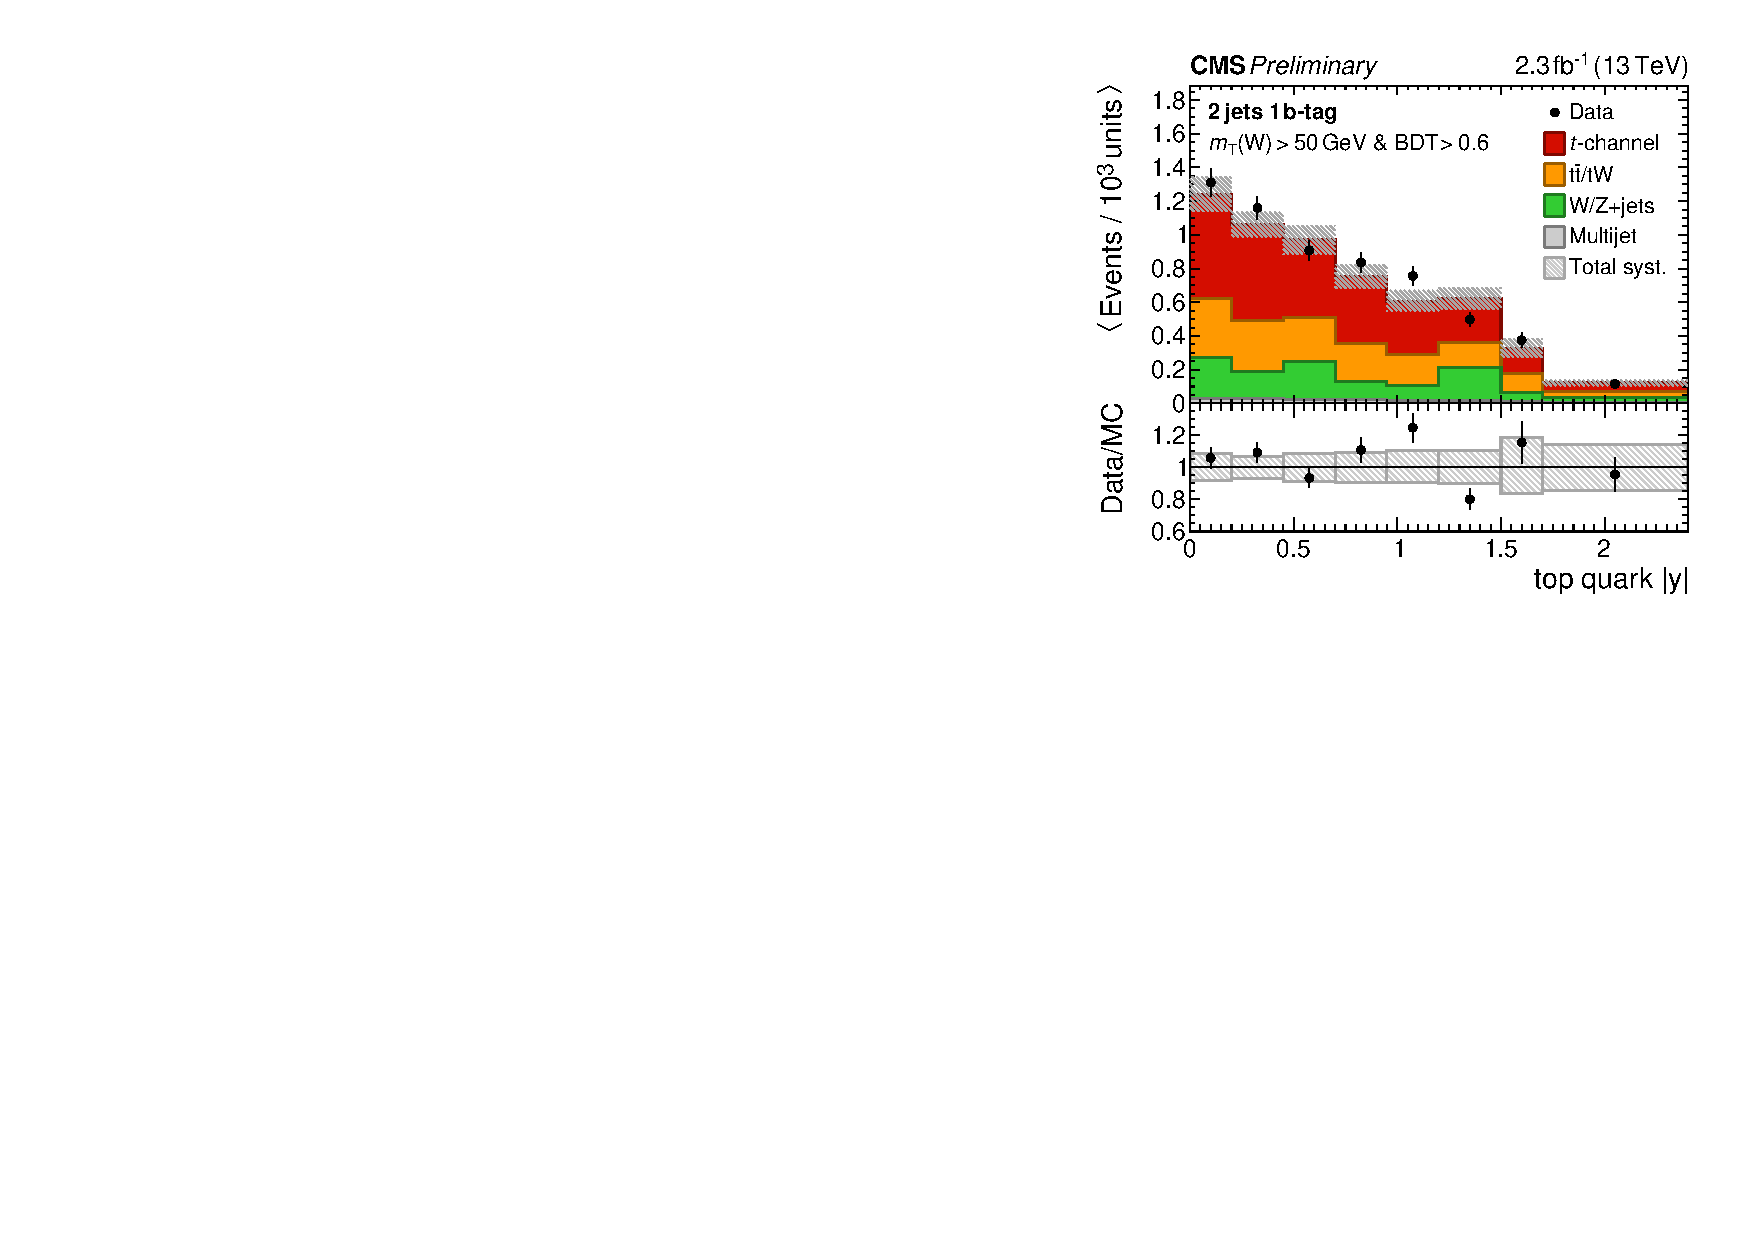
\includegraphics[width=0.48\textwidth]{figures/differential/pas/reco_topy_bdt.pdf}}
}

For a further cross check, the top quark \pt and rapidity distributions in the 3j1t \ttbar control region are shown in Fig.~\ref{fig:diff13-top-reco-3j1t}. Good agreement between data and simulation is observed for both distributions. Since no significant deviations are observed for the background modeling, the unfolding is performed to infer the differential cross sections at parton level.

\myfigure{\label{fig:diff13-top-reco-3j1t}Distributions of the (a)~top quark \pt and (b)~rapidity in the 3j1t control region.}{
\subfloat[]{\adjincludegraphics[height=4.8cm,trim={0 0 {0.16\width} 0},clip]{figures/differential/plots/3j1t/3j1t_top_pt_qcdnone_nol.pdf}}
\subfloat[]{\adjincludegraphics[height=4.8cm,trim={0 0 {0.\width} 0},clip]{figures/differential/plots/3j1t/3j1t_top_absy_qcdnone.pdf}}
}

%##############################################
\section{Unfolding}
%##############################################
\label{sec:diff13-unfolding}

The results obtained from the \gls{ml} fits are used to unfold the estimated distribution of $t$-channel single-top-quark events as a function of the top quark \pt and rapidity to parton level using the \TUNFOLD package. At reconstruction level the top quark \pt and rapidity are calculated from the summed 4-momenta of the selected b-tagged jet, muon and the reconstructed neutrino candidate. In particular the rapidity is calculated as $y=\frac{1}{2}\ln((E+p_{z})/(E-p_{z}))$ without utilizing knowledge about the top quark mass from other measurements. At parton level the top quark is defined to be on-shell while its momentum is also affected by boosts of the event induced by the simulation of \gls{qcd}/\gls{qed} radiations and by an intrinsic \kt of the initial-state partons. 

To find the optimal binning scheme for the unfolding, the migration of events between bins at reconstruction and parton level is studied. For this the stability $S$ and purity $P$, defined as 

\begin{equation}
S_{i}=\frac{\mathcal{R}_{ii}}{\sum\limits_{j}\,\mathcal{R}_{ij}}\,,\qquad P_{j}=\frac{\mathcal{R}_{jj}}{\sum\limits_{i}\,\mathcal{R}_{ij}}\,,
\end{equation}

are calculated from the response matrix $\mathcal{R}$ for various test-schemes. The stability denotes the amount of events generated in bin $i$ which do not migrate into other bins at reconstruction level. The purity on the other hand denotes the amount of events which have been reconstructed in bin $j$ but do not migrate into other bins at parton level. By choosing a suitable binning scheme for which both quantities are large (i.e. the migrations are low), less regularization has to be applied in the unfolding procedure. Hence, the procedure of finding such an optimized binning scheme is commonly considered as the first step for regularizing the ill-posed unfolding problem.

The final binning schemes chosen for the top quark \pt and rapidity at parton level are presented in Tab.~\ref{tab:diff13-ps-top} together with the calculated stabilities and purities per bin. Overall, both quantities are found to be above 50\% with the exception of the purity in the last rapidity bin which amounts to only 41\%. The corresponding response matrices are presented in Fig.~\ref{fig:diff13-response}. To stabilize the minimization procedure inside the \TUNFOLD method, eight bins are chosen at reconstruction level whereas only four bins are considered at parton level.

\mytable{\label{tab:diff13-ps-top}Stabilities and purities per bin of the top quark \pt and rapidity distribution at parton level.}{
\begin{tabular}{@{}l c c c c c@{}}

\toprule
Top quark \pt range     &  \hspace{0.3cm}   & \hspace{0.1cm}$0\range50~\GeV$\hspace{0.1cm} & \hspace{0.1cm}$50\range85~\GeV$\hspace{0.1cm} & \hspace{0.1cm}$85\range140~\GeV$\hspace{0.1cm} & \hspace{0.1cm}$140\range300~\GeV$ \\
\midrule
Stability &  &   59\% &     61\% &     64\% &     75\% \\
Purity &  &     63\% &     62\% &     63\% &     64\% \\
\midrule
\midrule
Top quark $|y|$ range  &  \hspace{0.3cm}     & \hspace{0.1cm}$0\range0.45$\hspace{0.1cm} & \hspace{0.1cm}$0.45\range0.95$\hspace{0.1cm} & \hspace{0.1cm}$0.95\range1.50$\hspace{0.1cm} & \hspace{0.1cm}$1.50\range2.40$ \\
\midrule
Stability & &    63\% &     54\% &     61\% &     86\% \\
Purity &    & 84\% &     57\% &     51\% &     41\% \\
\bottomrule
\end{tabular}
}



\myfigure{\label{fig:diff13-response}Response matrices for the top-quark (a)~transverse momentum and (b)~rapidity.}{
\subfloat[]{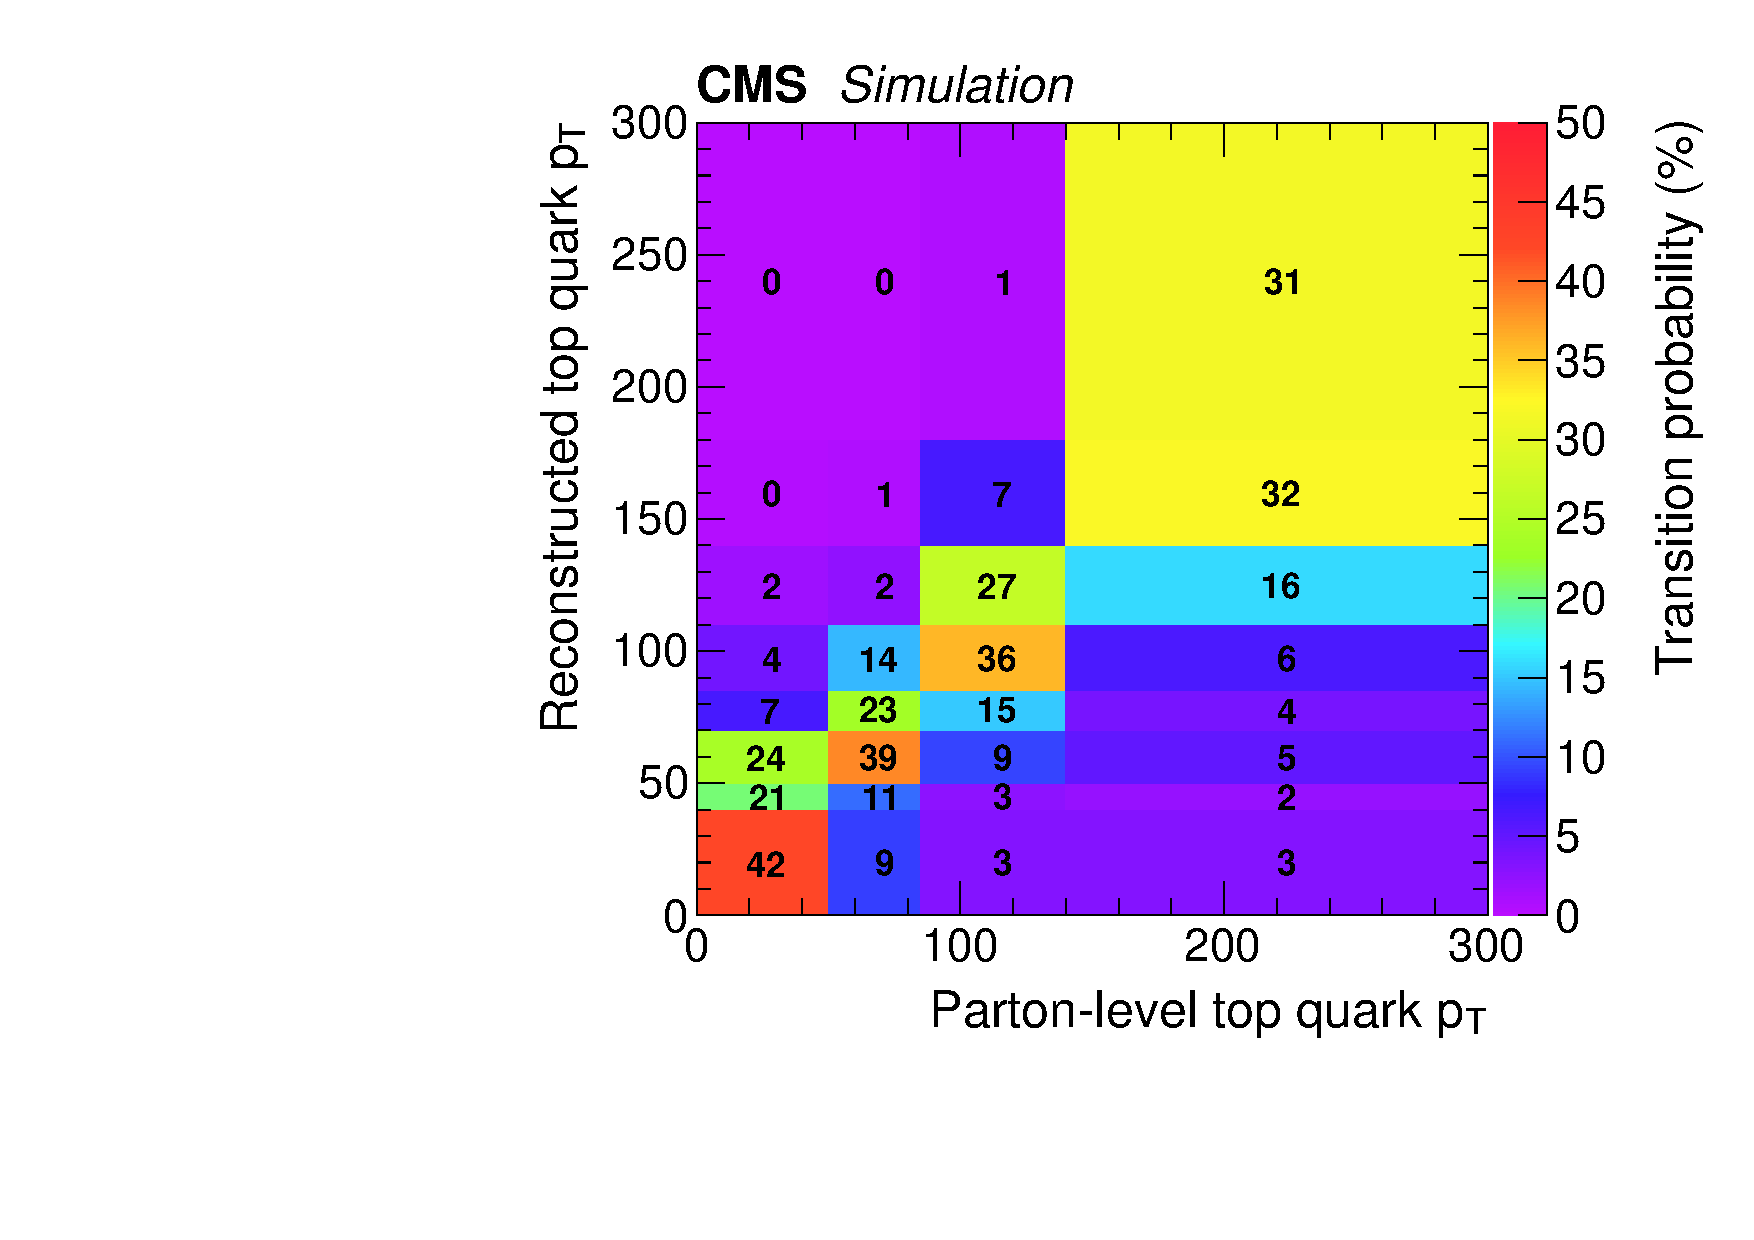
\includegraphics[width=0.48\textwidth]{figures/differential/unfolding/responsePt.pdf}}
\hspace{0.02\textwidth}
\subfloat[]{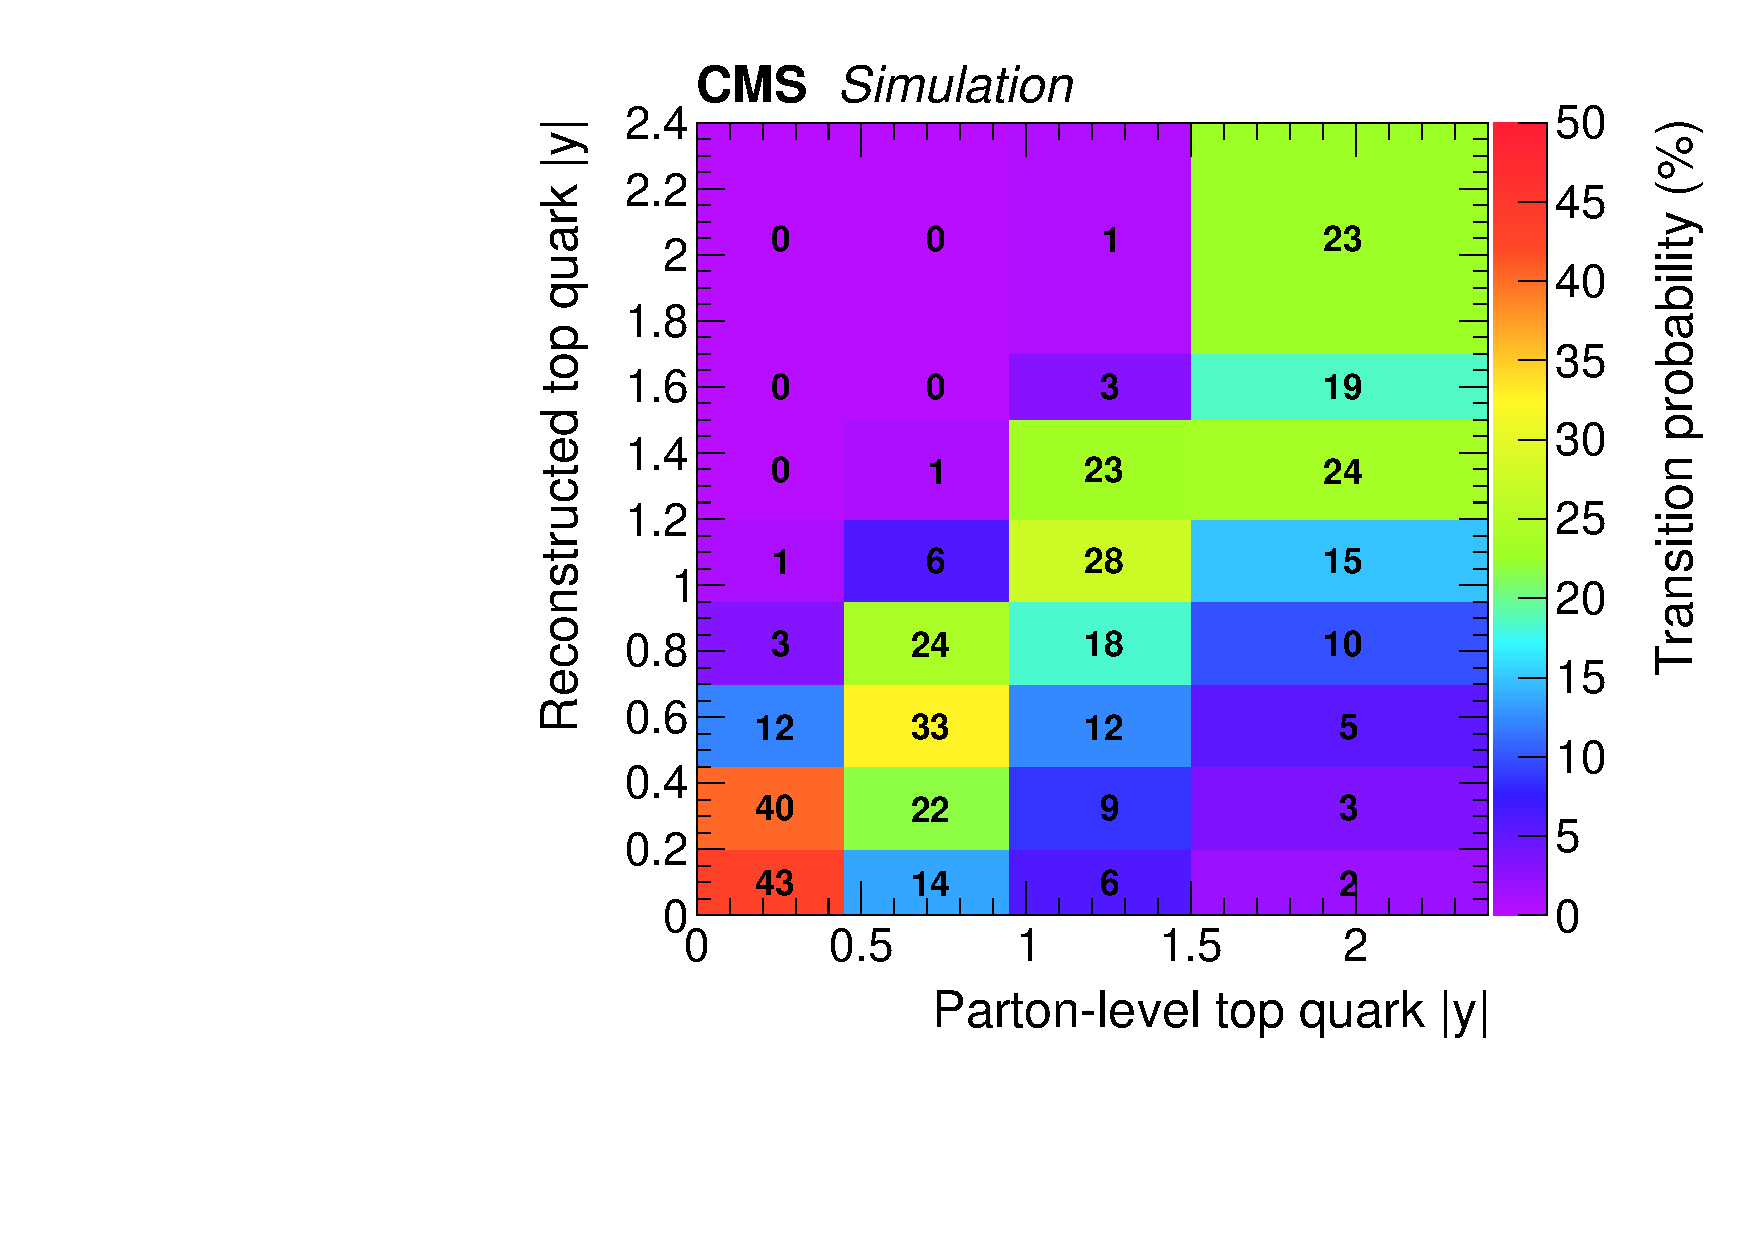
\includegraphics[width=0.48\textwidth]{figures/differential/unfolding/responseY.pdf}}
}

The selection efficiencies for $t$-channel single top quark events at reconstruction level with respect to parton level for the chosen binning schemes are also studied. They are presented in Fig.~\ref{fig:diff13-sel-efficiencies} after certain event selection steps as indicated. The efficiencies in the first top quark \pt bin and in the last rapidity bin are found to be relatively small ($\approx 1\%$)  compared to all other bins after selecting events in the 2j1t region together with $\mtw>50~\GeV$. Further optimization of the binning scheme at this stage would however degrade the obtained stability and purity and is therefore not envisaged.

\myfigure{\label{fig:diff13-sel-efficiencies}Selection efficiencies for the top-quark (a)~transverse momentum and (b)~rapidity.}{
\subfloat[\label{fig:diff13-sel-efficiencies-pt}]{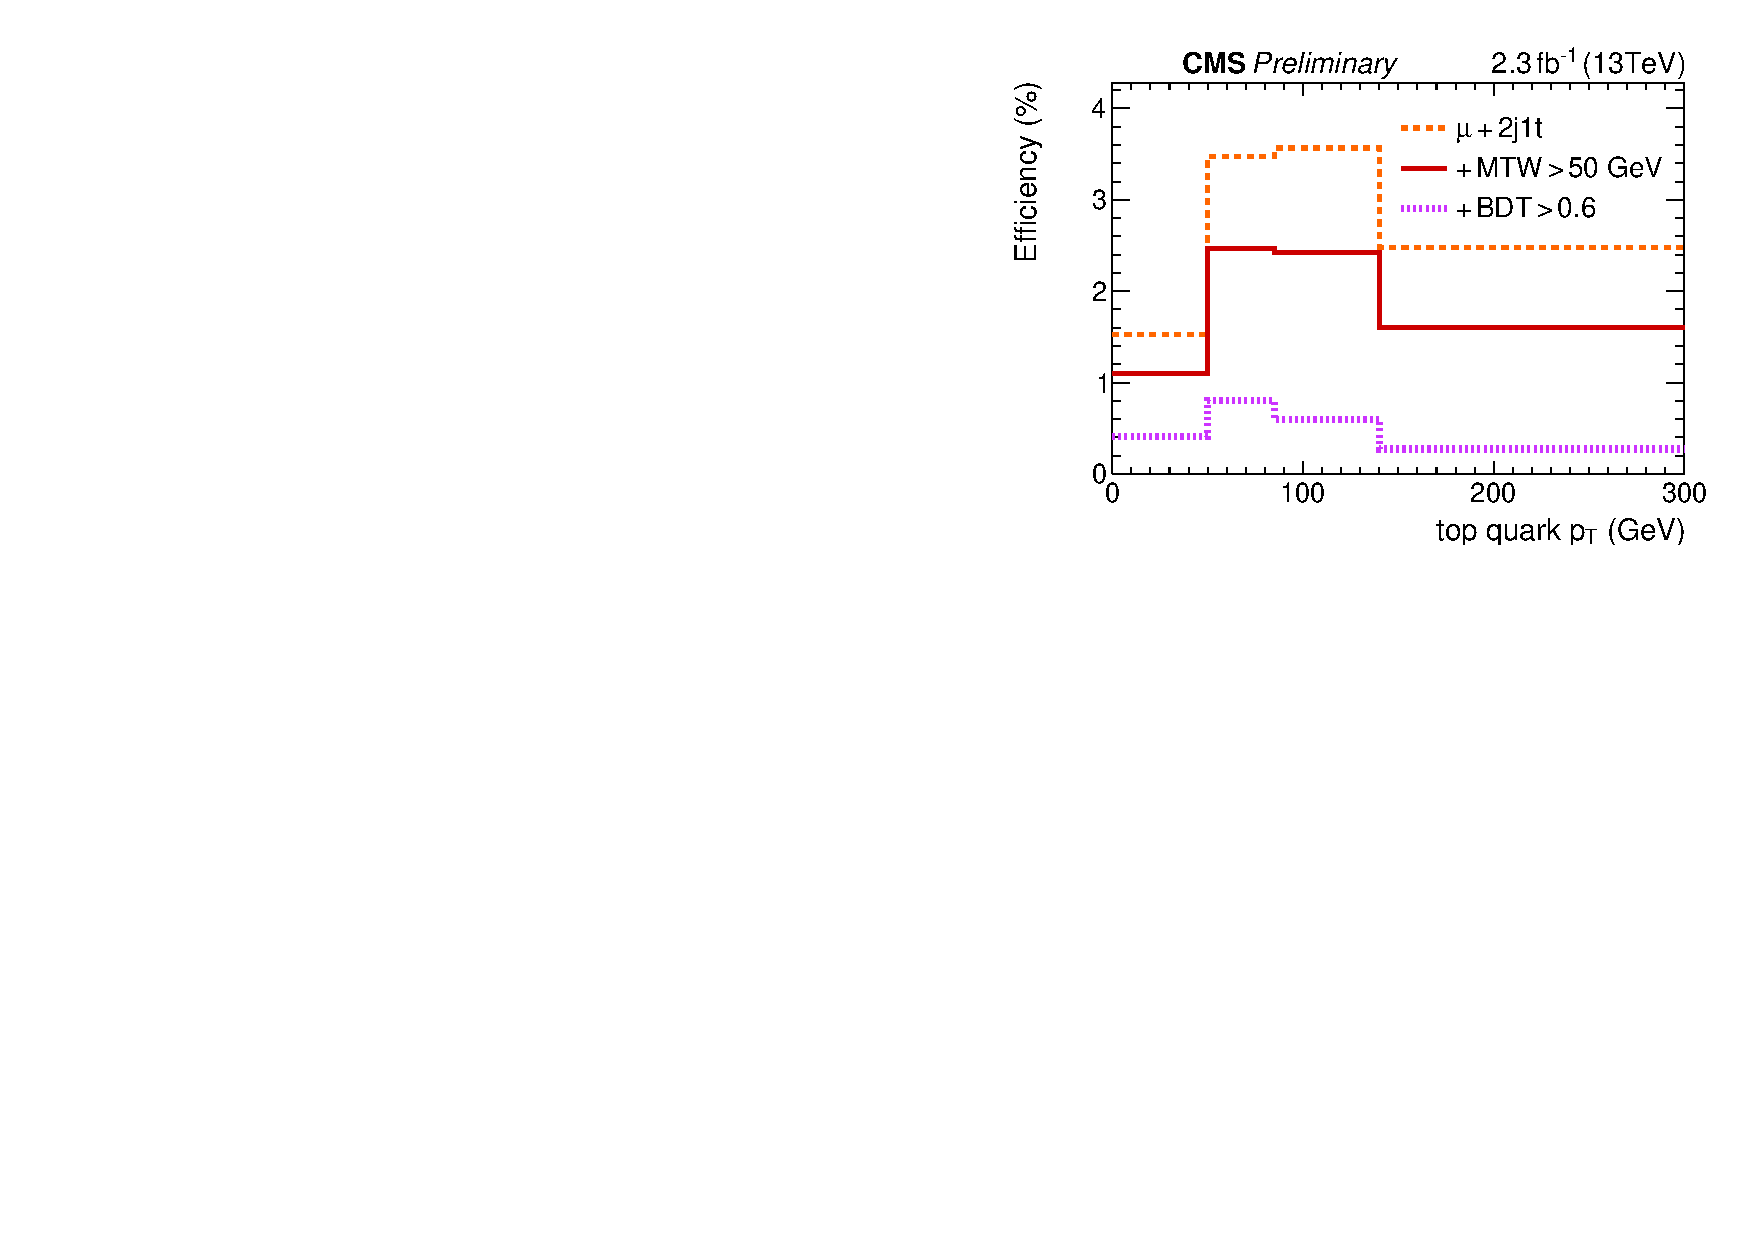
\includegraphics[width=0.48\textwidth]{figures/differential/unfolding/effPt.pdf}}
\hspace{0.02\textwidth}
\subfloat[]{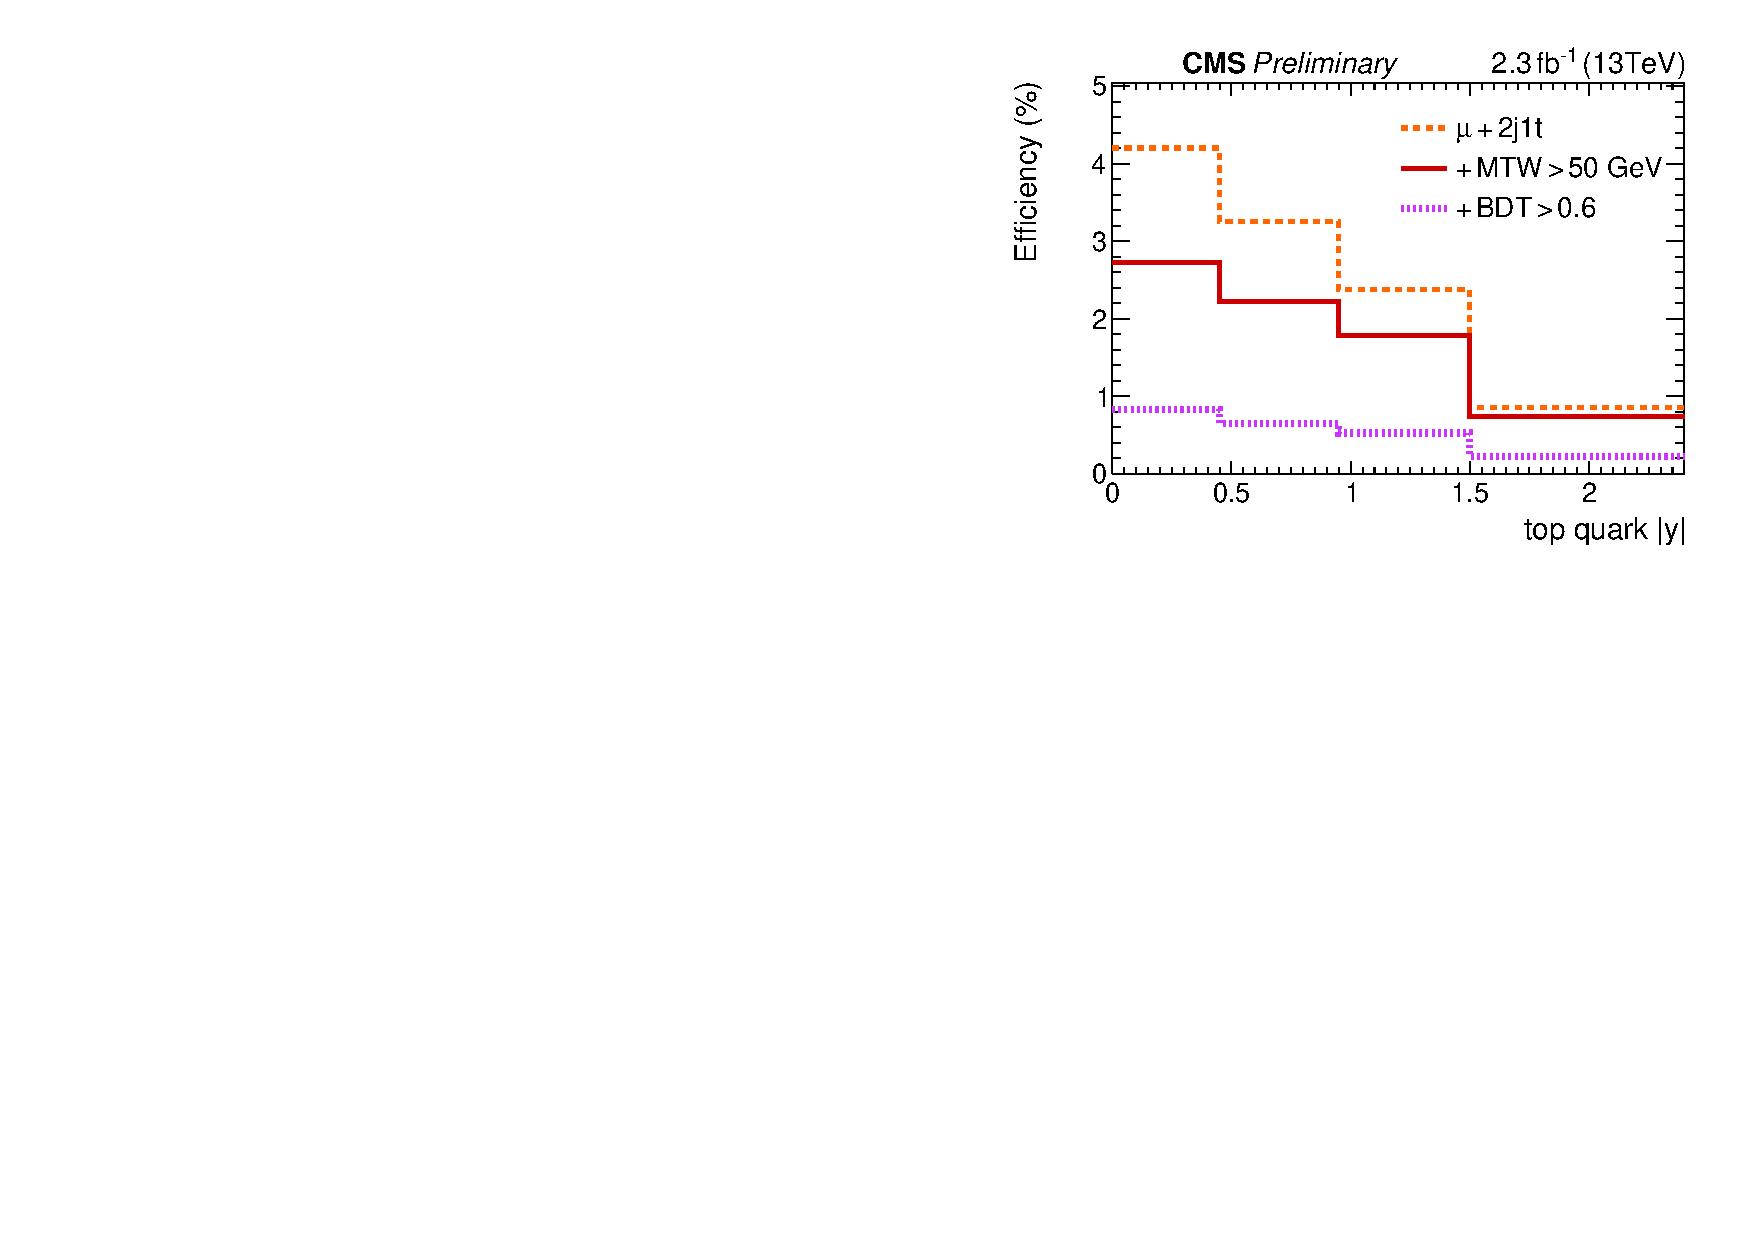
\includegraphics[width=0.48\textwidth]{figures/differential/unfolding/effY.pdf}}
}


%##############################################
\section{Statistical evaluation}
%##############################################

The measurement is affected by various sources of systematic uncertainties. For each source new templates are derived which reflect a systematic variation by one standard deviation. Those are then propagated through the fitting procedure, the \gls{bdt} evaluation, and the unfolding. Special care is taken in the unfolding step since not only the templates can change under a systematic variation but also the response matrices themselves. To calculate the resulting differential cross section, pseudo experiments are performed by dicing normal distributions per uncertainty source around the nominal spectrum. The resulting yields $y_{i}^\mathrm{total}$ per bin $i$ can be express as

\begin{equation}
y_{i}^\mathrm{total}=y_{i}^\mathrm{nominal}+\mathsf{N}\Big(0,\mathcal{V}^\mathrm{stat.}\Big)_{i}+\sum_{j}^\mathrm{sources}\,\mathsf{N}\Big(0,\,\Delta^{\mathrm{\pm syst.\,}j}_{i}\Big)\,,
\end{equation}

where $\mathsf{N}$ denotes the normal distribution, $\mathcal{V}^\mathrm{stat.}$ the covariance matrix of the statistical uncertainty, and $\Delta^\scriptn{\mathrm{\pm syst.\,}j}_{i}$ the differences in yields between the shifted and nominal templates per systematic source $j$. From the distribution of the yields over many pseudo experiments, the central value of the differential cross section is taken to be the median and its uncertainty is quoted as the quantile corresponding to one standard deviation. In the following the considered sources of systematic uncertainties are briefly described.

\begin{description}
\item[Background composition] In the \gls{ml} fits the \zjets and tW templates are grouped together with the larger \wjets and \ttbar templates respectively. To assess the impact of the assumed ratios on the measurement, their contributions to the fit templates are varied conservatively by $\pm20\%$ independently.
 
\item[Multijet template] An uncertainty on the extract multijet template is taken into account by assessing the impact on the measurement when using two alternative templates derived from subregions in the muon isolation of either $[20\%; 40\%]$ or $[40\%; \infty]$ instead as detailed in Sec.~\ref{sec:diff13-selection}.

\item[Analysis objects] A summary of the considered sources of systematic uncertainties related to the reconstruction and selection of analysis objects is provided in Sec.~\ref{sec:reconstruction-summary}. This includes uncertainties on the jet energy scale and resolution, b-tagging and mistagging efficiencies, muon trigger, identification, and isolation efficiencies, and the pileup reweighting.

\item[Signal and hadronization modeling] The modeling of signal events generated with \MGAMC is assessed by comparing to the result obtained when using a sample generated with \POWHEG instead. Additionally, a sample generated with \MGAMC interfaced with \HERWIG is used to assess the dependence of the result on the hadronization model.

\item[Top quark mass] Dedicated samples of $t$-channel, tW, and \ttbar events are generated to account for an conservative uncertainty of $172.5\pm1.0~\GeV$ on the top quark mass.

\item[\Acrlong{pdf}] The uncertainty on the \gls{pdf} is assessed by reweighting the simulated samples according to the 102 variations of the NNPDF3.0 set~\cite{Ball:2014uwa}.

\item[Renormalization and factorization scales] The uncertainty on the renormalization scale is propagated to the result by performing a reweighting procedure of simulated \ttbar, tW, \wjets, and $t$-channel events according to the scale dependence of the corresponding \acrlongpl{me}. Additionally, the factorization scale is varied by using dedicated samples. The final uncertainty is taken to be the envelope of varying both scales independently by a factor of two or one-half with respect to the nominal scale choice with the exception of extreme up/down combinations.

\item[\ttbar \pt reweighting] The \ttbar \pt reweighting has been applied by default in this measurement since it improves the agreement of the prediction with data at 13~TeV similar to Sec.~\ref{sec:polarization-modeling}. A corresponding uncertainty is assessed by rederiving the result without applying the reweighting.
\end{description}

The sources of systematic uncertainties with a relatively large impact on the measurement are shown in Figs.~\ref{fig:diff13-top-sys-pt} and~\ref{fig:diff13-top-sys-y} per top quark \pt and rapidity bin. Some of the largest ones are the data statistics ($\approx10\range25\%$), the renormalization and factorization scale choice ($\approx10\range15\%$), the top quark mass ($\approx5\range20\%$), and the jet energy scale and resolution ($\approx5\range15\%$). Especially the first top quark \pt bin is affected heavily by most uncertainties which is also related to the low acceptance of signal events in this particular bin as presented in Fig.~\ref{fig:diff13-sel-efficiencies-pt}. Additionally, a large uncertainty in this bin is also expected from theory originating from differences between the predictions in the 4~or 5~\gls{fs} as discussed in Sec.~\ref{sec:theory-flavor-schemes}.

\myfigure{\label{fig:diff13-top-sys-pt} Relative impact on the yield for some of the largest systematic uncertainties on the measured top quark \pt spectrum. The dashed vertical lines mark the bin edges.}{
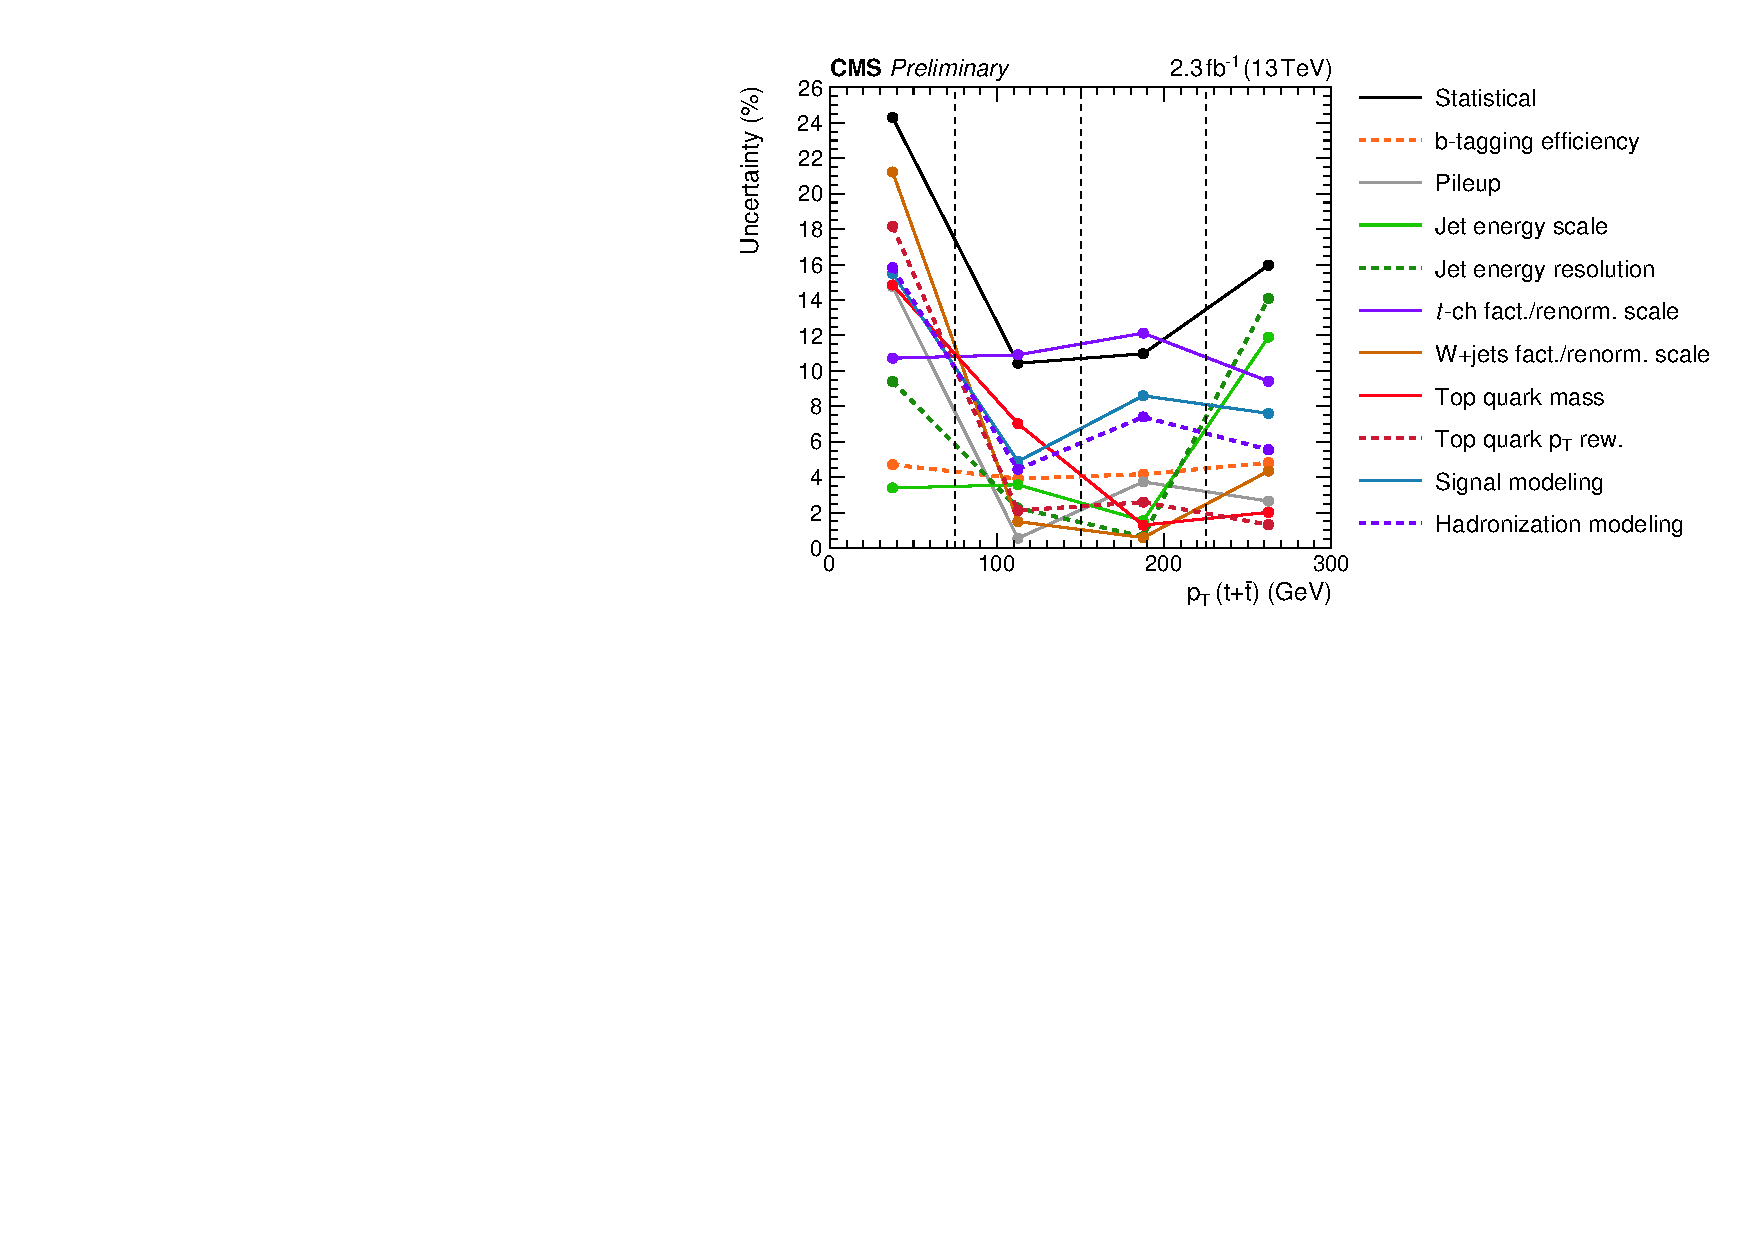
\includegraphics[width=0.9\textwidth]{figures/differential/unfolding/unfolded_top_pt_unc.pdf}
}

\myfigure{\label{fig:diff13-top-sys-y} Relative impact on the yield for some of the largest systematic uncertainties on the measured top quark rapidity spectrum. The dashed vertical lines mark the bin edges.}{
\subfloat[]{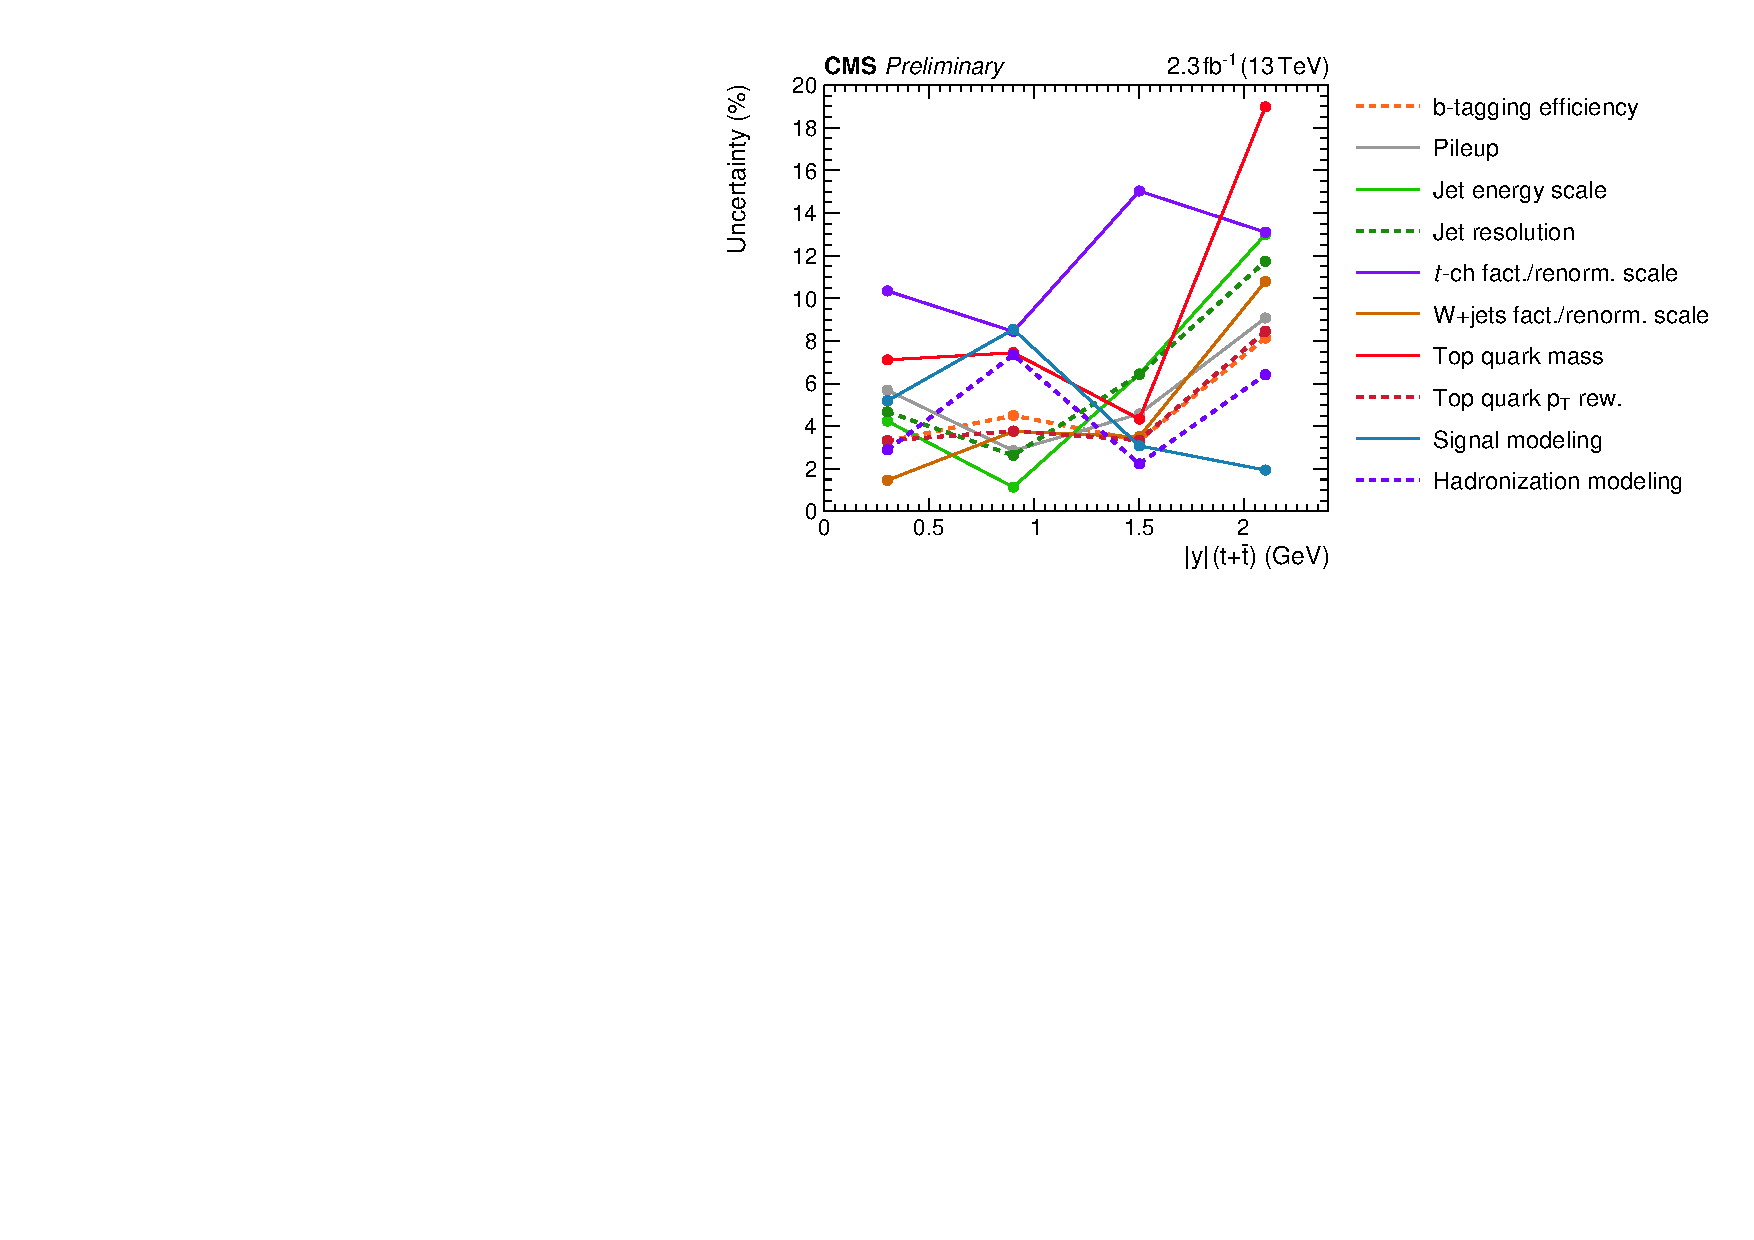
\includegraphics[width=0.9\textwidth]{figures/differential/unfolding/unfolded_top_y_unc.pdf}}
}

%##############################################
\section{Results}
%##############################################

The measured normalized differential cross sections as a function of the top quark \pt and rapidity are presented in Fig.~\ref{fig:diff13-top-unfolded}. The spectra are compared to the \gls{sm} predictions by \MGAMC interfaced with \PYTHIA in 4~\gls{fs}, \POWHEG interfaced with \PYTHIA in 4~\gls{fs}, \MGAMC interfaced with \PYTHIA in 5~\gls{fs}, and \MGAMC interfaced with \HERWIG in 4~\gls{fs}. Overall the results agree with the predictions within uncertainties. In particular, the first top quark \pt bin is found to be affected by uncertainties at large leading to a total relative uncertainty of about $\pm50\%$ which renders the observed deviation with respect to the predictions not very significant.

\myfigure{\label{fig:diff13-top-unfolded}The measured normalized differential cross section of $t$-channel single-top-quark production as a function of the top quark (a)~\pt and (b)~rapidity. The statistical uncertainties are indicated by horizontal ticks on the error bars. The figures are taken from Ref.~\cite{CMS-PAS-TOP-16-004}.}{
\subfloat[]{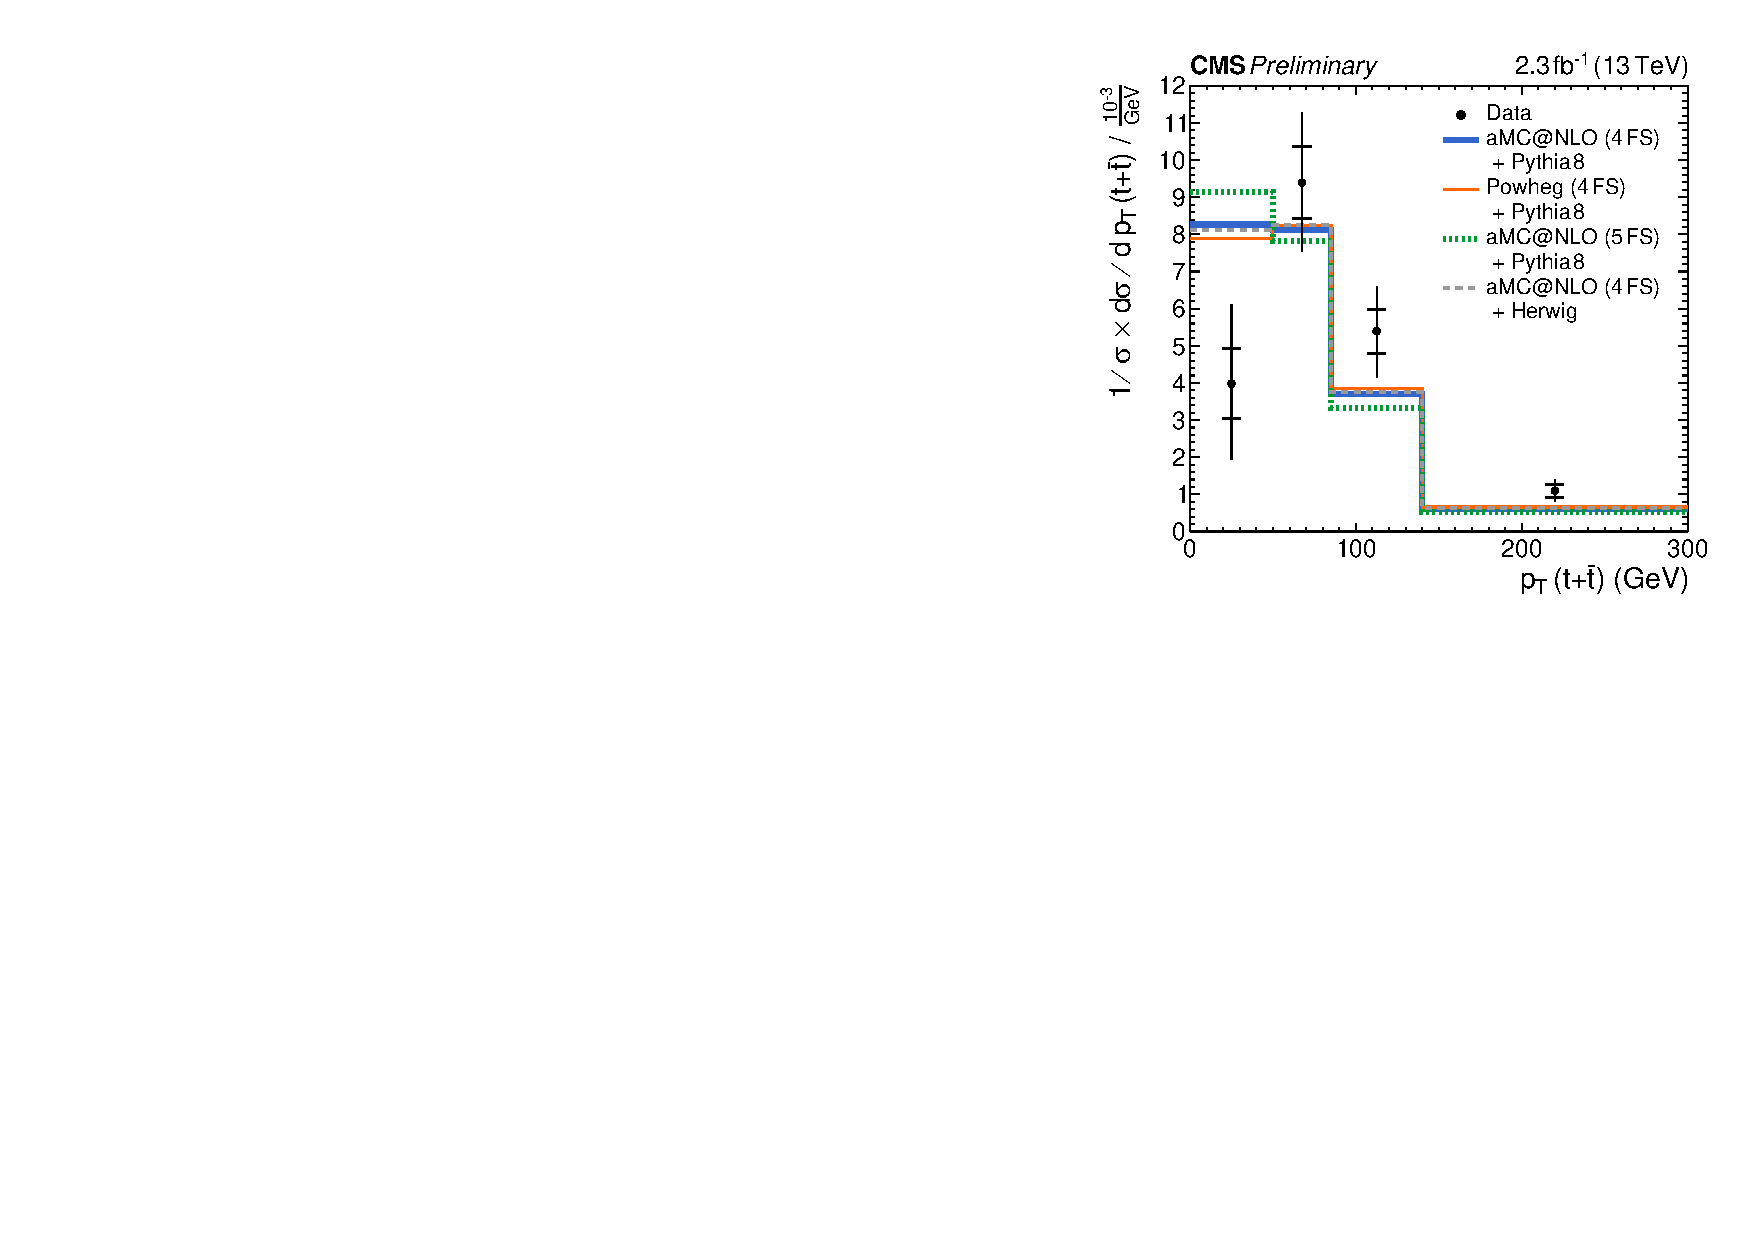
\includegraphics[width=0.48\textwidth]{figures/differential/pas/unfolded_top_pt.pdf}}
\hspace{0.02\textwidth}
\subfloat[]{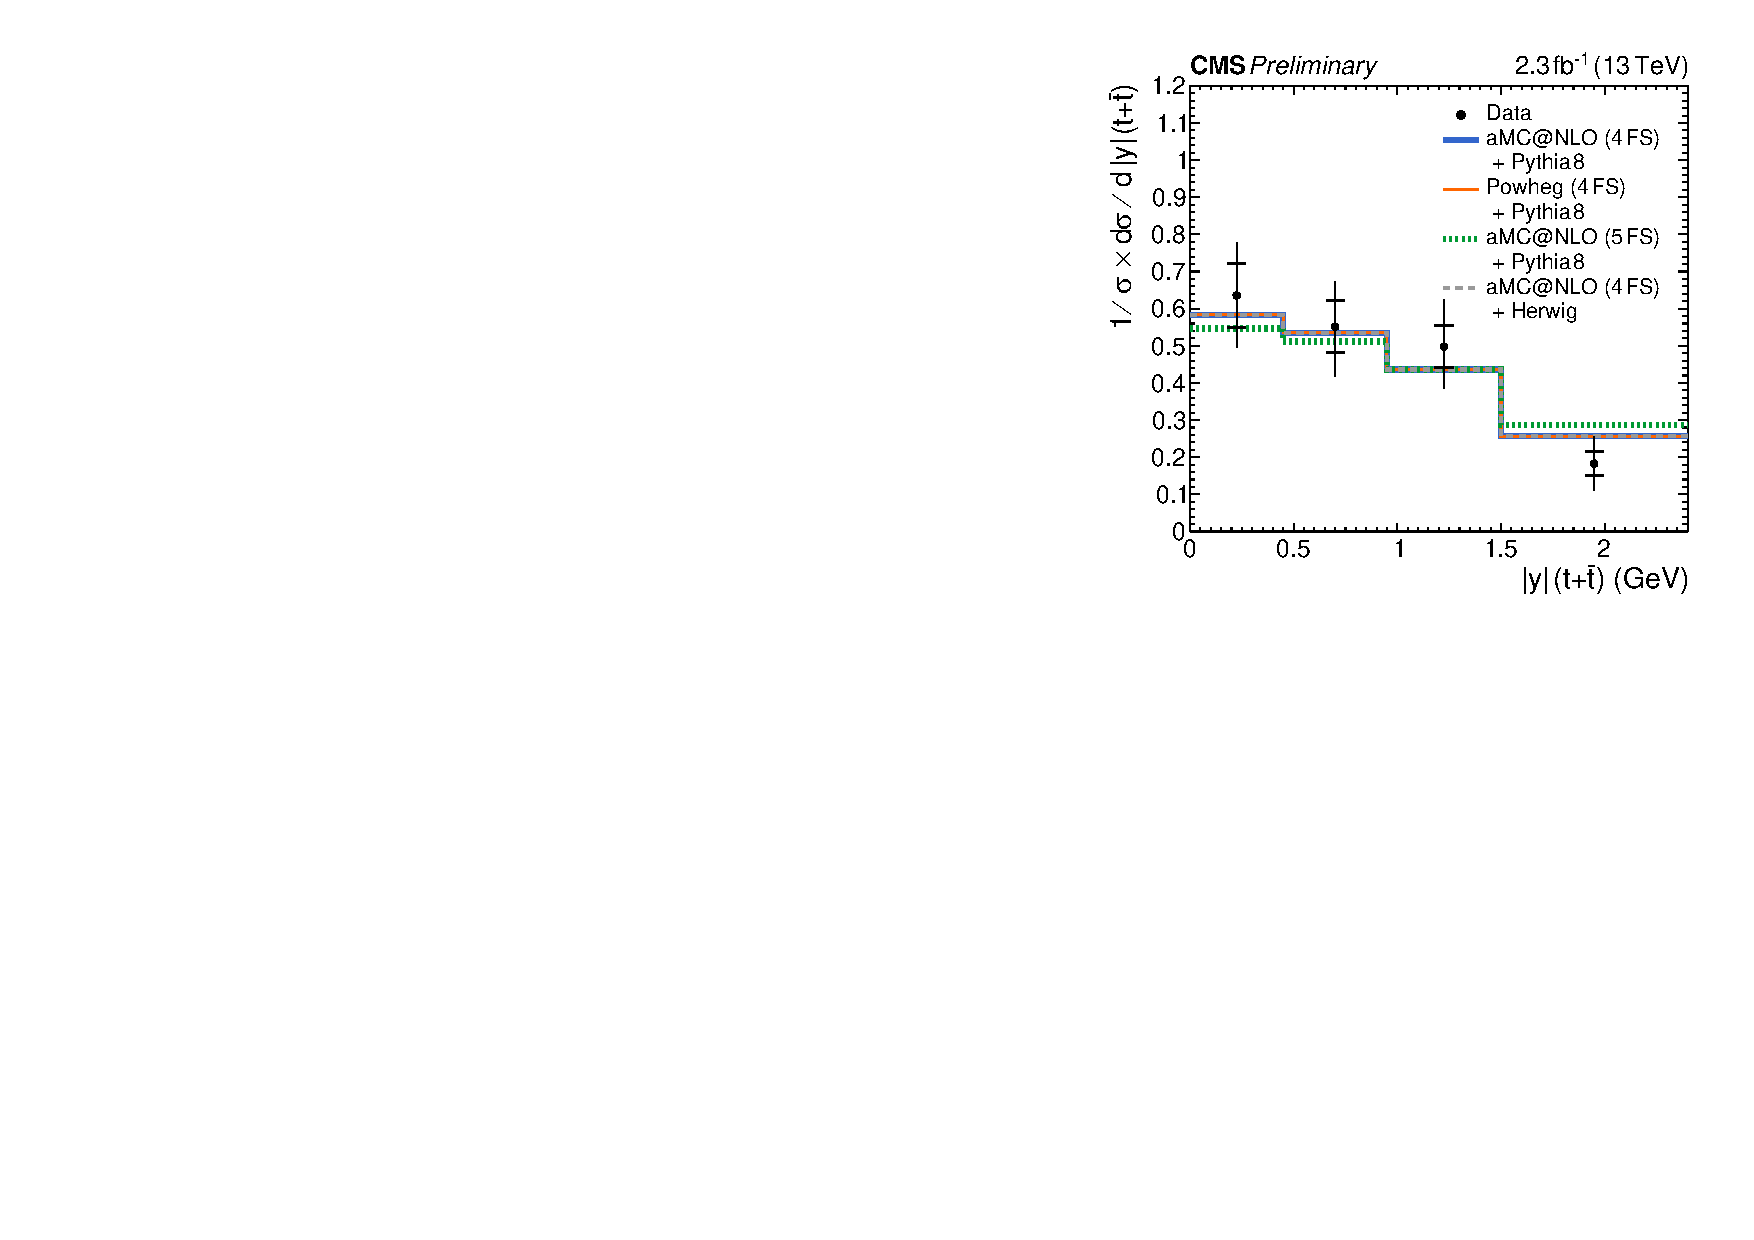
\includegraphics[width=0.48\textwidth]{figures/differential/pas/unfolded_top_y.pdf}}
}

To cross check the result of the top quark \pt spectrum, the measurement has been repeated by fitting the distribution of the pseudorapidity of the spectator jet~(Fig.~\ref{fig:diff13-training-obs-etaj}) instead of the \gls{bdt} distribution. The resulting differential cross section is presented in Fig.~\ref{fig:diff13-top-unfolded-xcheck}. It confirms the obtained result within however larger uncertainties.

\myfigure{\label{fig:diff13-top-unfolded-xcheck}Cross check of the top quark \pt differential cross section result by fitting the pseudorapidity distribution of the spectator jet instead of the \gls{bdt} discriminant. The statistical uncertainties are indicated by horizontal ticks on the error bars.}{
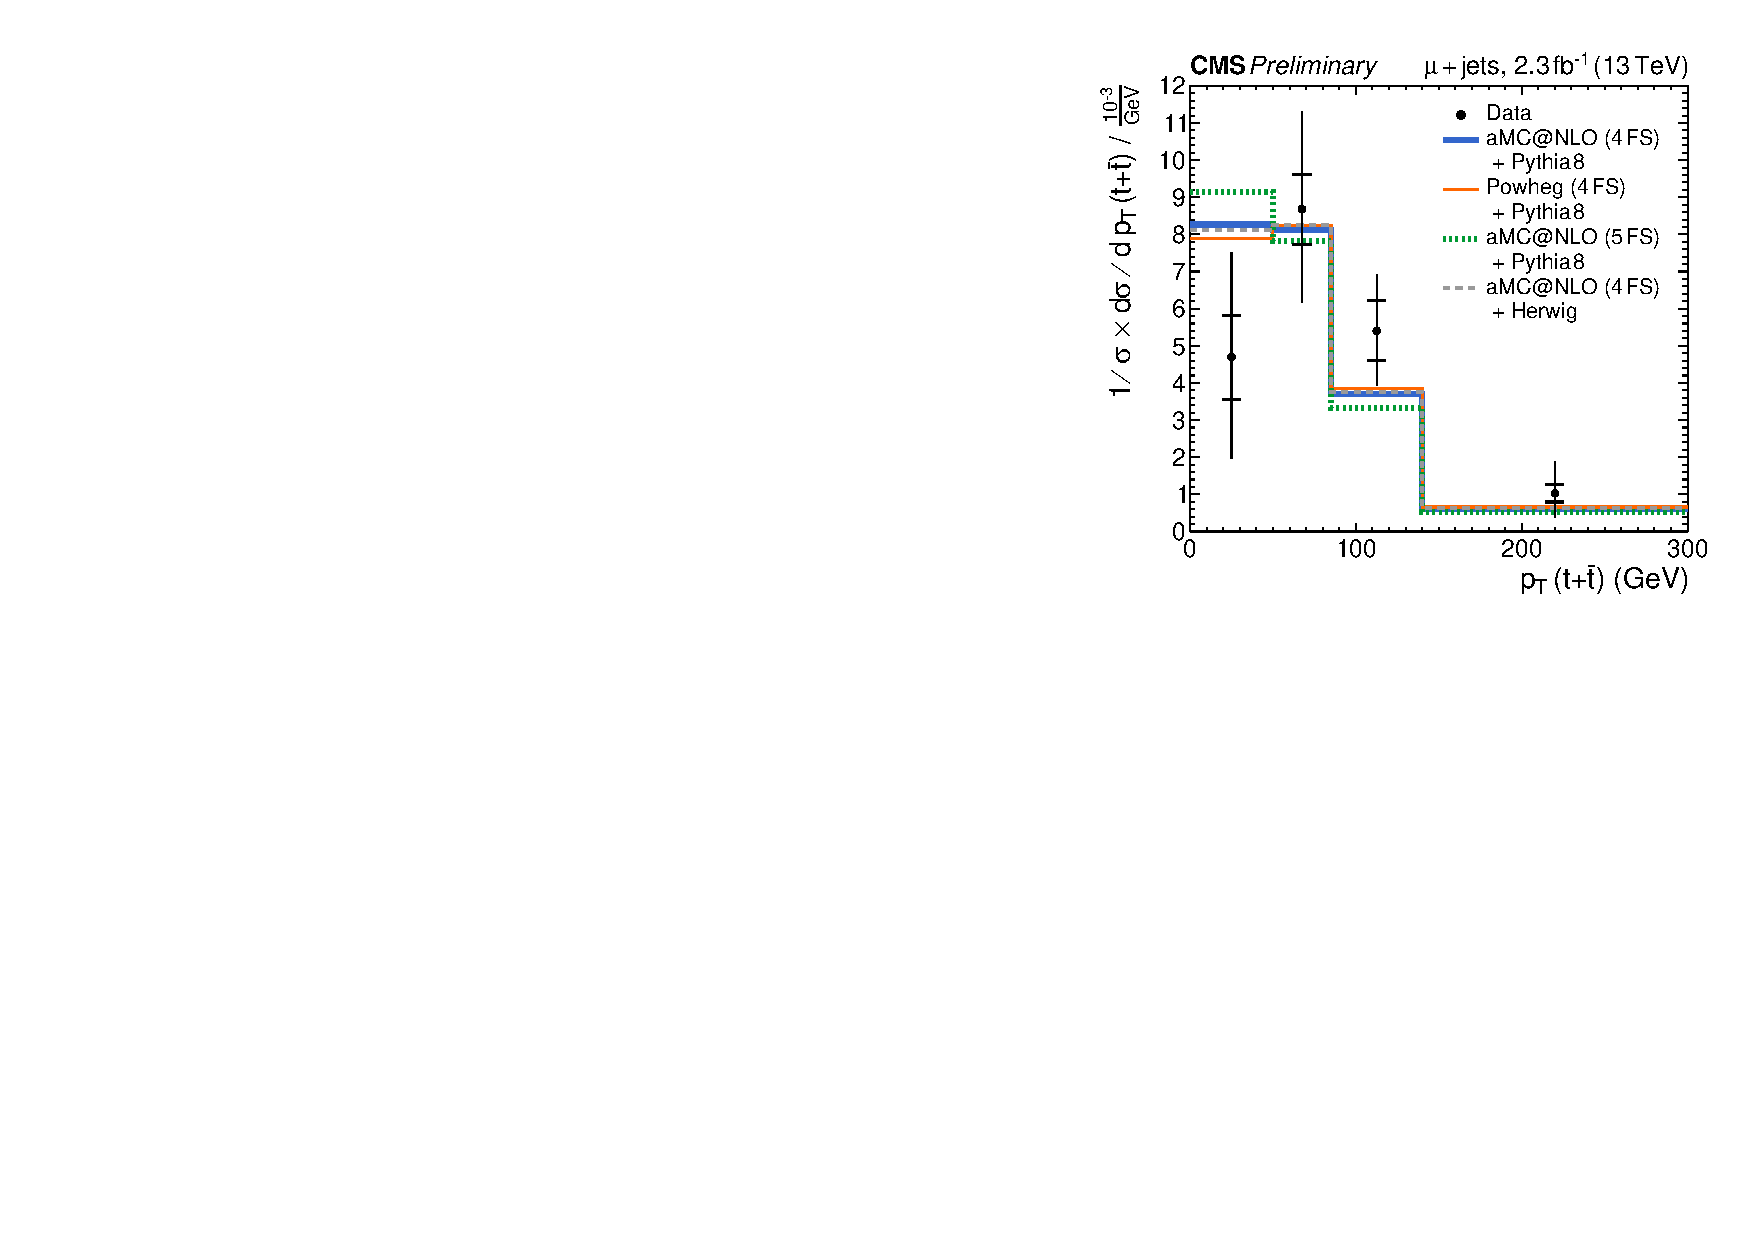
\includegraphics[width=0.48\textwidth]{figures/differential/pas/unfolded_top_pt_jeta.pdf}
}

